\chapter{PRÉSENTATION ET DISCUSSION DES RÉSULTATS SUR LES APPRENTISSAGES}

Ce chapitre présente l'ensemble des résultats des expérimentations.  Il se divise en trois volets principaux:

\begin{enumerate}
    \item La présentation et l'analyse de l'apprentissage;
    \item La présentation et l'analyse des résultats de l'application des modèles pour l'estimation des paramètres polarimétriques sur les données synthétiques.
    \item La présentation des résultats de l'application des modèles sur les données réelles.
\end{enumerate}

Nous discuterons des résultats en familles de modèles ou ensembles de modèles pour un même nombre de blocs résiduels $m$ et un même nombre de filtres par convolution $p$.  Chacune de ces familles comportes 7 modèles en lien avec la taille $n$ de la première convolution. Nous ne présenterons pas tous les résultats individuels, car ils seraient trop nombreux. Nous pourrons les consulter dans les annexes.  Nous donnons un condensé permettant de tirer des conclusions sur l'ensemble des résultats.

\section{L'analyse de l'apprentissage}

Les apprentissages ont été produits selon le protocole expérimental expliqué à la Section \ref{sec:experimental_protocol}. L'objectif n'était pas de trouver les paramètres susceptibles de produire des modèles optimaux mais de minimiser les effets susceptibles d'influencer les résultats, par exemple nous avons toujours utilisé le même taux d'apprentissage $\lambda$ pour toutes les expérimentations. Les tableaux suivants (Tab.  \ref{tab:homogeneous_training}, Tab.  \ref{tab:heterogeneous_training} et Tab.  \ref{tab:heterogeneous_training_with_targets}) comptabilisent le nombre des apprentissages produits pour chacun des ensembles de données simulées décrits aux Sections \ref{sec:simulation_de_region_homomgene} et \ref{section:simulation_heterogeneous_regions}.  Au total nous avons produit 154 modèles en faisant varier les paramètres de l'architecture \acrconvnet décrite à la Section \ref{sec:description_cnn}.  Nous avons modulé sur certaines plages, le nombre $m$ de blocs résiduels, le nombre $p$ de filtres par convolution et la taille $n$  des filtres de la première couche convolutive du \acrconvnet.  

Le temps d'exécution d'un apprentissage a été en moyenne de 11.9 heures $\pm$ 4.4 heures et le nombre total d'heures machine est estimé à 1833 heures, soit environ 76.3 jours. L'utilisation d'un cluster \acrgpu au CRIM\footnote{Centre de Recherche Informatique de Montréal, ww.crim.ca} a donc été primordiale pour la réussite du projet.  Il a permis de réduire le temps machine en exécutant plusieurs apprentissages en parallèle.  La Figure \ref{fig:processing_time} présente les temps d'exécution pour la série d'apprentissages correspondant à l’ensemble $m={0,1,3,5}$ et $p=8$.  De manière générale le temps dépend de la taille du modèle et du type de carte graphique. Les temps au-dessous de 5 heures comptabilisent seulement le temps suite à une reprise pour finaliser un entraînement qui avait échoué.  Dans ces cas d'échec, l'entraînement du modèle est repris à l'époque $t$ du dernier modèle valide et est poursuivi jusqu'à l'époque finale $t=150$. Les temps supérieurs à 20 heures montrent que le cluster a été surchargé, c'est-à-dire que la charge au niveau des CPU était excessive parce qu'il y avait trop de tâches par CPU. Ce qui provoque une dégradation au niveau de la performance car le transfert des données entre le CPU et le \acrgpu est limité par la vitesse du CPU. 

\vspace{5mm}

\begin{table}[!htbp]
\tiny
\centering
\begin{tabular}{|c|c|c|c|c|c|}
\hline
    \textbf{m/p}            & \textbf{8}             & \textbf{16}            & \textbf{32}            & \textbf{64}            & \textbf{total} \\ \hline
\textbf{0}     & \textbf{n}=\{3,5,7,9,11,13,15\} & \textbf{n}=\{3,5,7,9,11,13,15\} & \textbf{n}=\{3,5,7,9,11,13,15\} & \textbf{n}=\{3,5,7,9,11,13,15\} & 28 modèles    \\ \hline
\textbf{1}     & \textbf{n}=\{3,5,7,9,11,13,15\}                        &                        &                        &                        &       7 modèles          \\ \hline
\textbf{3}     & \textbf{n}=\{3,5,7,9,11,13,15\}                        &                        &                        &                        &       7 modèles         \\ \hline
\textbf{5}     & \textbf{n}=\{3,5,7,9,11,13,15\}                        &                        &                        &                        &       7 modèles         \\ \hline
\textbf{total} & 28  modèles                         &    7 modèles                    &   7 modèles                      &      7 modèles        &    49 modèles           \\ \hline
\end{tabular}
\caption{\small{
Ensemble des apprentissages produits à partir des \textbf{données simulées homogènes} en fonction de la paramétrisation de la structure du réseau de neurones. Le nombre de blocs résiduels est donné par $m$, le nombre de filtres par convolution est donné par $p$ et la taille de l'entrée de la première convolution est donnée par $n$.
}
}
\label{tab:homogeneous_training}
\end{table}

\begin{table}[!htbp]
\tiny
\centering
\begin{tabular}{|c|c|c|c|c|c|}
\hline
    \textbf{m/p}            & \textbf{8}             & \textbf{16}            & \textbf{32}            & \textbf{64}            & \textbf{total} \\ \hline
\textbf{0}     & \textbf{n}=\{3,5,7,9,11,13,15\} & \textbf{n}=\{3,5,7,9,11,13,15\} & \textbf{n}=\{3,5,7,9,11,13,15\} & \textbf{n}=\{3,5,7,9,11,13,15\} & 28 modèles    \\ \hline
\textbf{1}     & \textbf{n}=\{3,5,7,9,11,13,15\}                        &                        &                        &                        &     7 modèles           \\ \hline
\textbf{3}     & \textbf{n}=\{3,5,7,9,11,13,15\}                        &                        &                        &                        &       7 modèles         \\ \hline
\textbf{5}     & \textbf{n}=\{3,5,7,9,11,13,15\}                        &                        &                        &                        &       7 modèles          \\ \hline
\textbf{total} & 28  modèles                     &   7 modèles                     &    7 modèles                     &   7 modèles                      &    49 modèles            \\ \hline
\end{tabular}
\caption{\small{
Ensemble des apprentissages produits à partir des \textbf{données simulées hétérogènes} en fonction de la paramétrisation de la structure du réseau de neurones. Le nombre de blocs résiduels est donné par $m$, le nombre de filtres par convolution est donné par $p$ et la taille de l'entrée de la première convolution est donnée par $n$.
}
}
\label{tab:heterogeneous_training}
\end{table}

\begin{table}[!htbp]
\tiny
\centering
\begin{tabular}{|c|c|c|c|c|c|}
\hline
    \textbf{m/p}            & \textbf{8}             & \textbf{16}            & \textbf{32}            & \textbf{64}            & \textbf{total} \\ \hline
\textbf{0}     & \textbf{n}=\{3,5,7,9,11,13,15\} & \textbf{n}=\{3,5,7,9,11,13,15\} & \textbf{n}=\{3,5,7,9,11,13,15\} & \textbf{n}=\{3,5,7,9,11,13,15\} & 28 modèles    \\ \hline
\textbf{1}     & \textbf{n}=\{3,5,7,9,11,13,15\}                        &                        &                        &                        &          7 modèles      \\ \hline
\textbf{3}     & \textbf{n}=\{3,5,7,9,11,13,15\}                        &                        &                        &                        &          7 modèles      \\ \hline
\textbf{5}     & \textbf{n}=\{3,5,7,9,11,13,15\}                        &                        &                        &   \textbf{n}=\{3,5,7,9,11,13,15\}   &          14 modèles       \\ \hline
\textbf{total} & 28  modèles                         &  7 modèles                       & 7  modèles                      &       14 modèles                 &    56 modèles             \\ \hline
\end{tabular}
\caption{\small{
Ensemble des apprentissages produits à partir des \textbf{données simulées hétérogènes avec l'inclusion de cibles ponctuelles} en fonction de la paramétrisation de la structure du réseau de neurones. Le nombre de blocs résiduels est donné par $m$, le nombre de filtres par convolution est donné par $p$ et la taille de l'entrée de la première convolution est donnée par $n$.
}
}
\label{tab:heterogeneous_training_with_targets}
\end{table}

\begin{figure}[!htbp] 
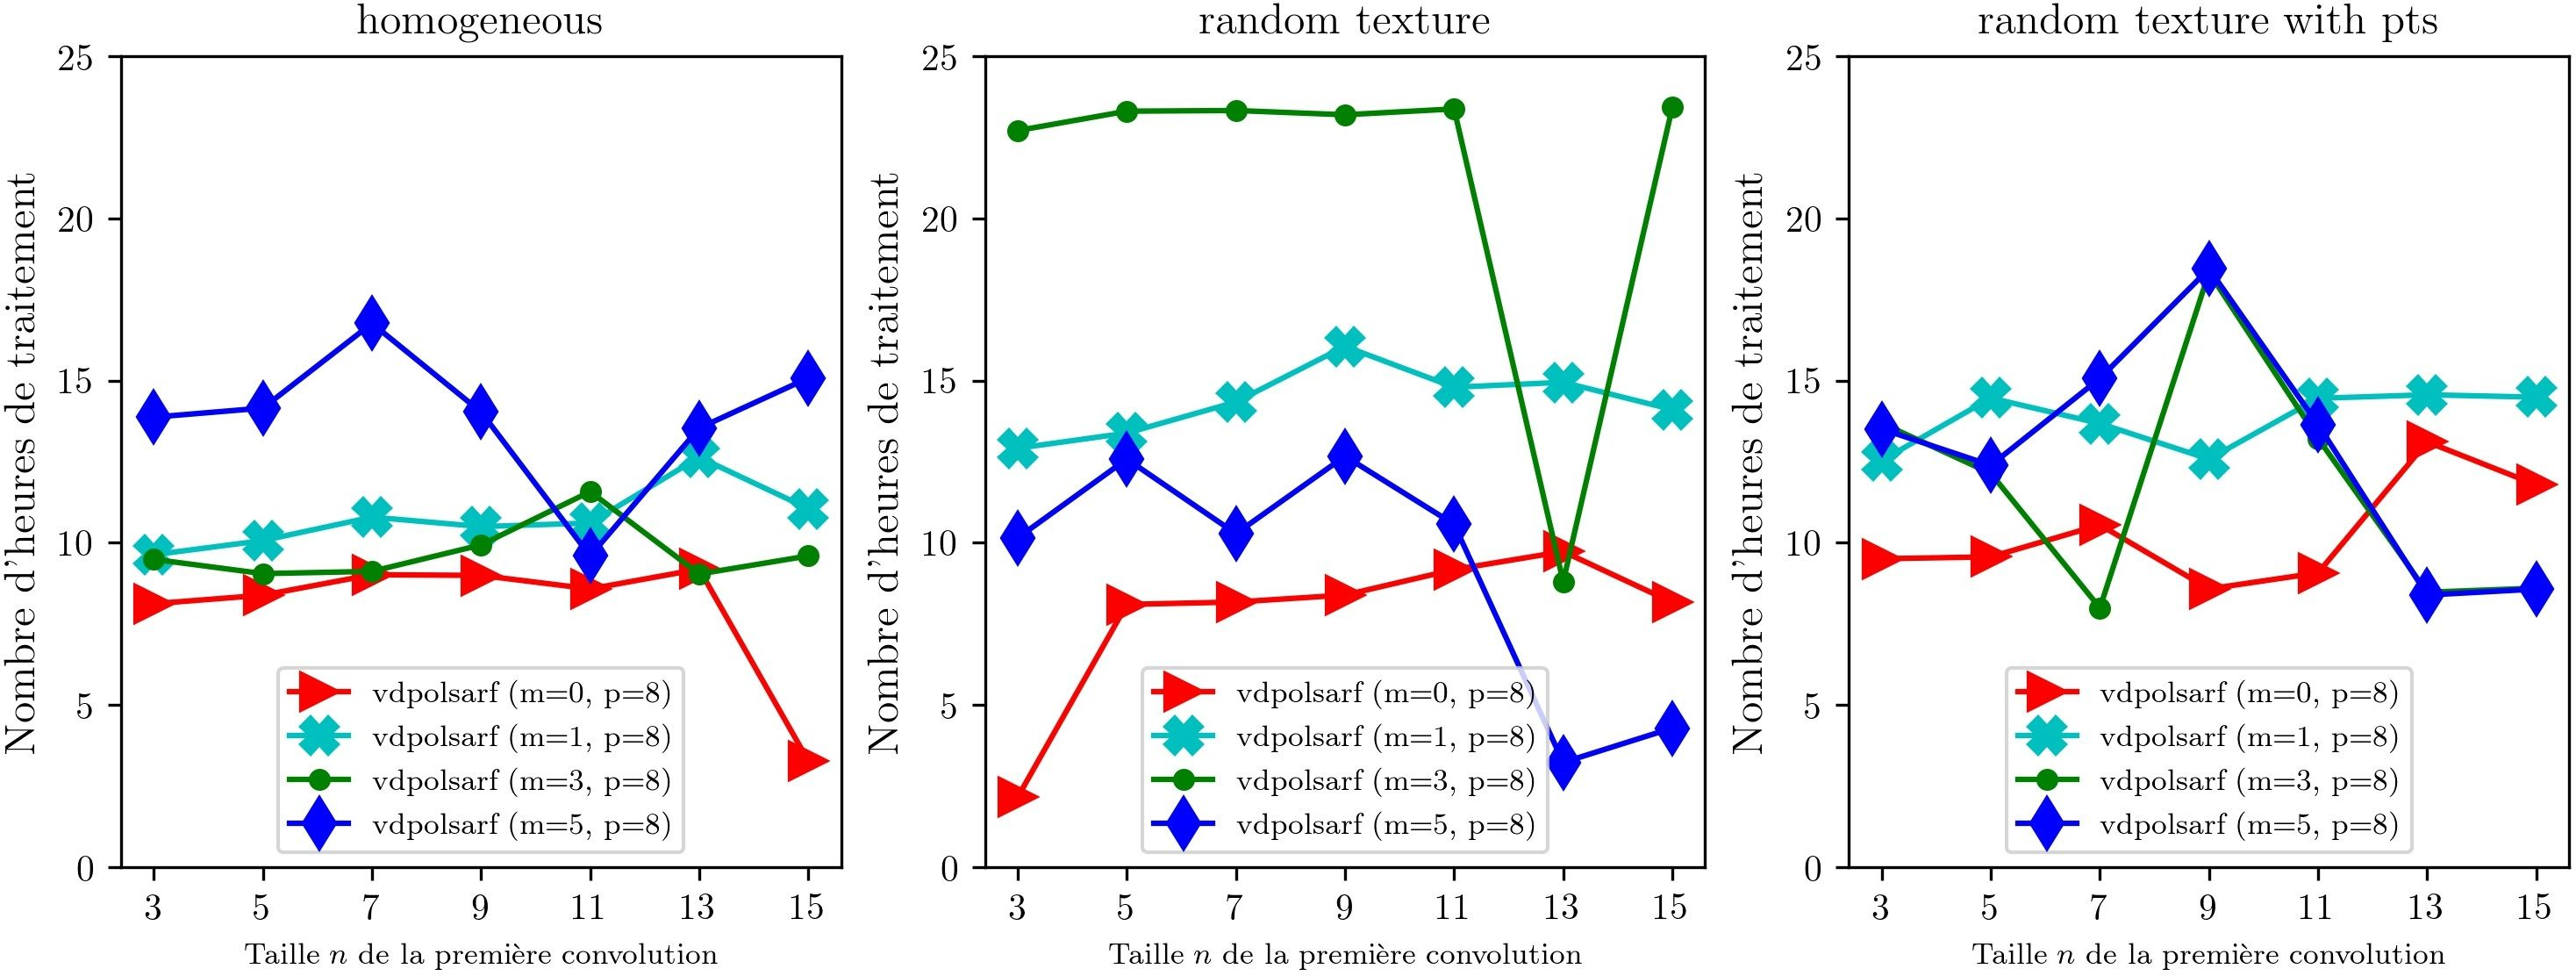
\includegraphics[width=1.0\textwidth]{figures/Chap4/results/processing_time.jpg}
 \centering
  \caption{
  \small{Temps d'exécution des apprentissages de l'ensemble des $m=\{0,1,3,5\}$ et $p=8$. La figure de gauche présente les temps pour l'apprentissage sur les données homogènes.  La figure centrale montre le temps pour l'apprentissage sur les données hétérogènes et la figure de gauche montre celui pour les données hétérogènes avec inclusion de cibles ponctuelles. Nombre totale d'apprentissage = 84. Nombre d'heures total = 1003.4 heures. Temps moyen d'un apprentissage = 11.9 heures $\pm$ 4.4 heures.}
  }
  \label{fig:processing_time}
\end{figure}

\begin{figure}[!htbp] 
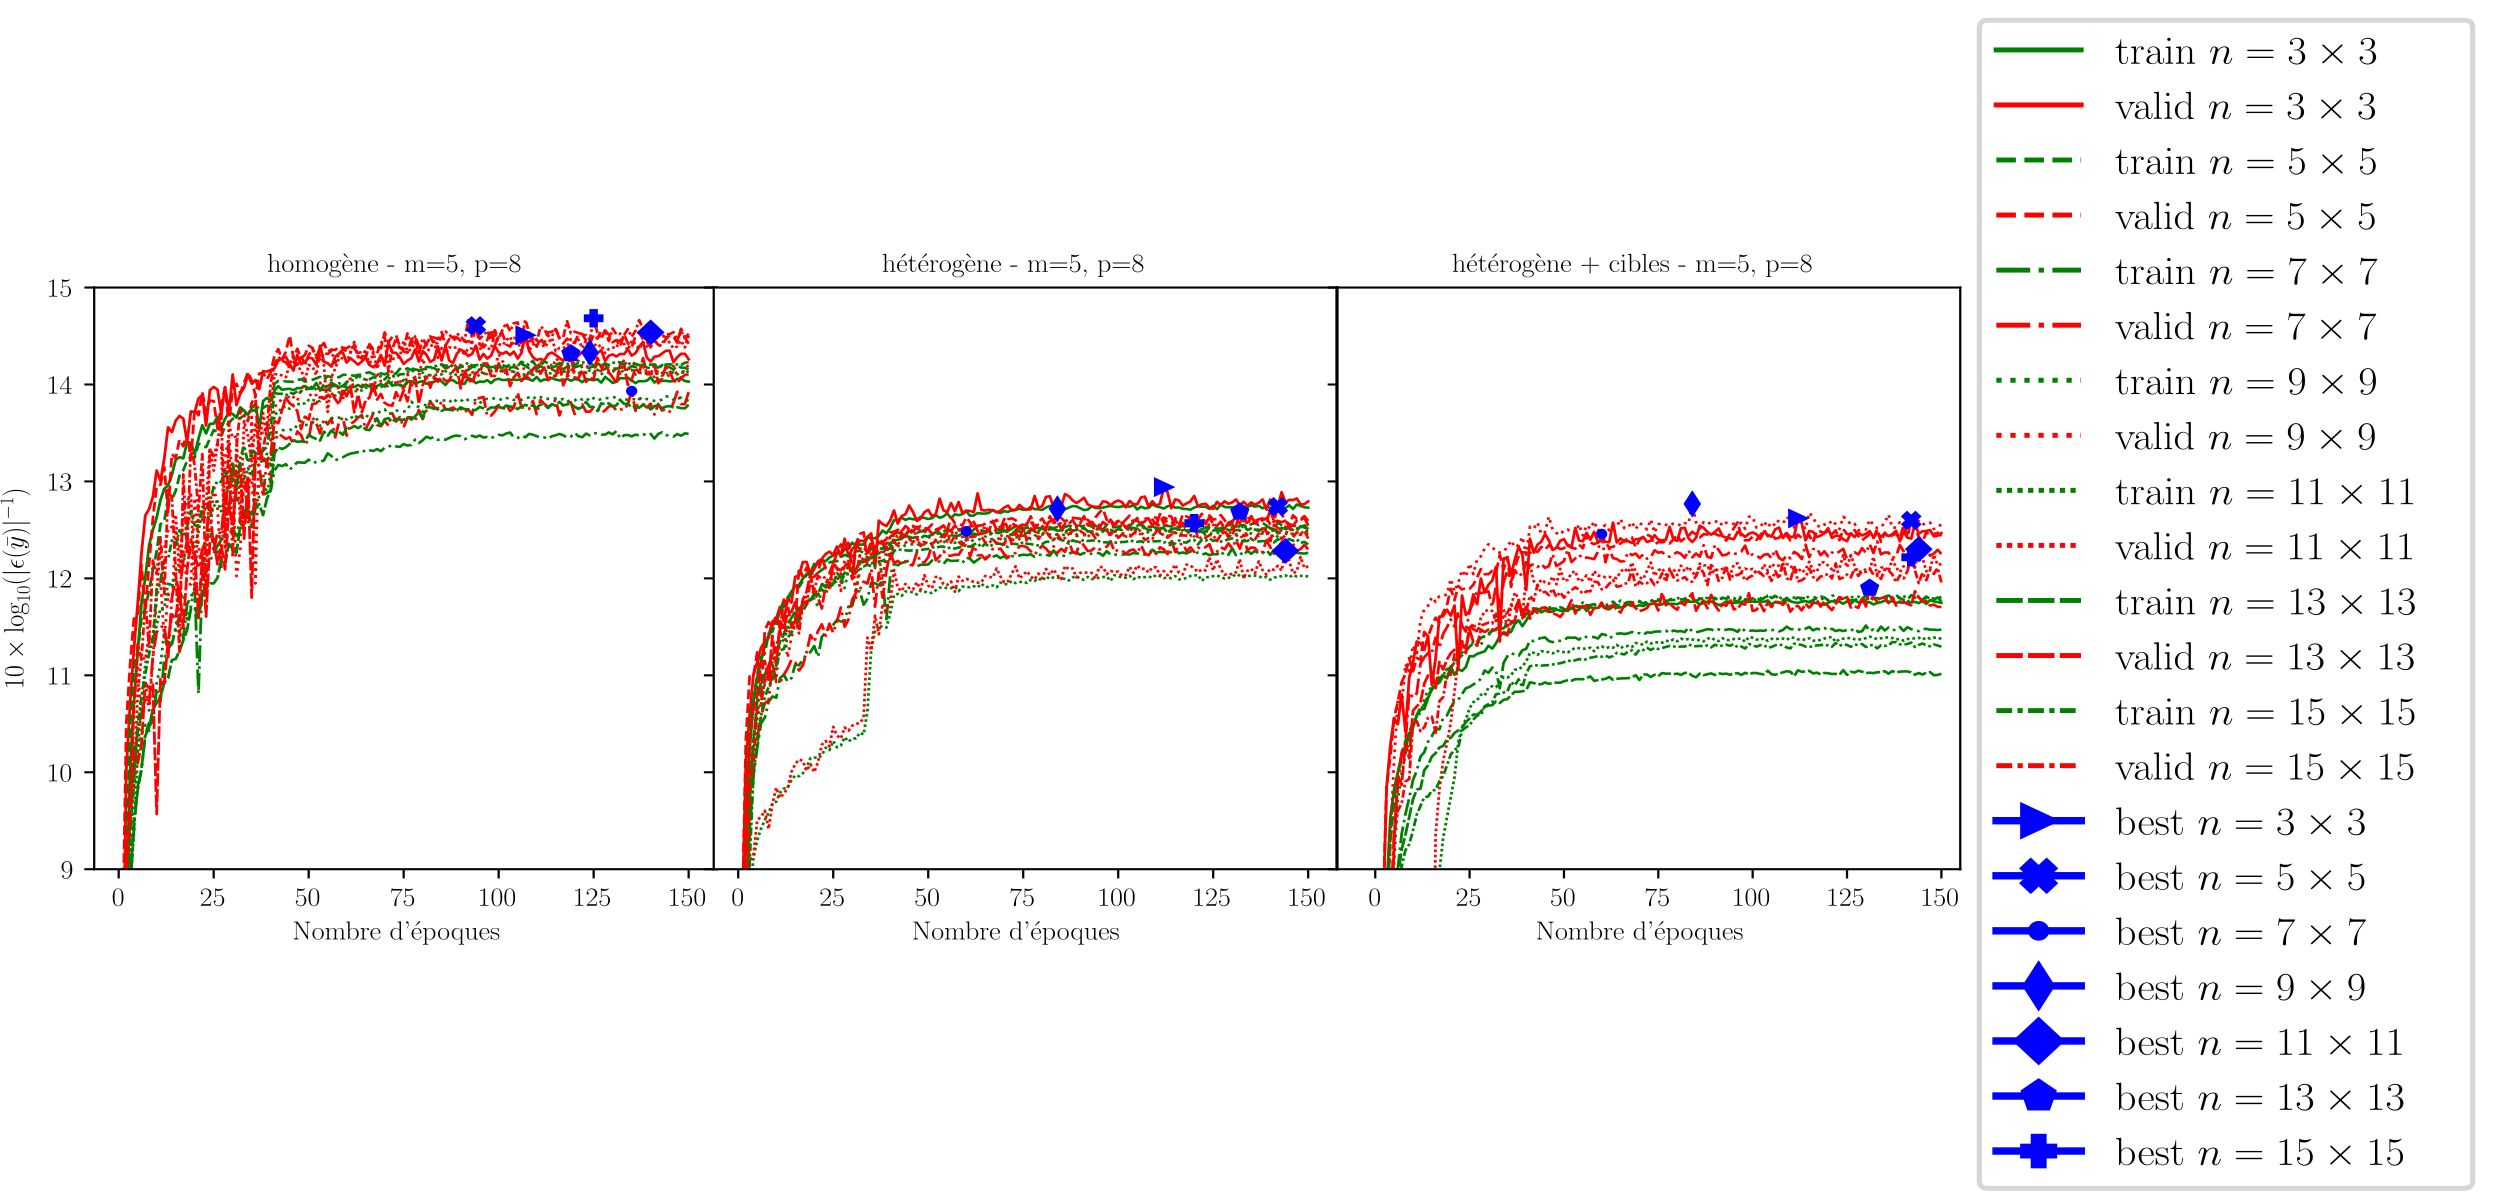
\includegraphics[width=1.20\textwidth, angle=270,origin=c]{figures/Chap4/results/training_types_compare/training_curves_m=5_p=8_n=all.jpg}
 \centering
  \caption{
  \small{Exemple de courbes d'apprentissage sur la famille $m=5$, $p=8$ montrant l'erreur d'apprentissage en fonction du nombre d'époques (\textcolor{green}{vert} = entraînement, \textcolor{red}{rouge}  = validation, \textcolor{blue}{bleu}  = meilleurs modèles). La figure de gauche présente les résultats relatif à l'apprentissage des modèles sur l'ensemble de données homogènes.  La figure centrale montre les résultats pour l'apprentissage sur les données hétérogènes et la figure de gauche montre celui pour les données hétérogènes avec inclusion de cibles ponctuelles.}
  }
  \label{fig:training_curves_m=5_p=8_n=all}
\end{figure}

La Figure \ref{fig:training_curves_m=5_p=8_n=all} présente les courbes de l'erreur de l'apprentissage sur l'ensemble des modèles $m=\{0,1,3,5\}$ et $p=8$ en fonction du nombre d'époques pour nos trois types d'entraînement. Il est à noter que l'erreur absolue $|\epsilon|$ est représentée par son inverse sous une échelle logarithmique en base 10 pour faciliter l'interprétation des résultats en fonction des époques finales. L'erreur sur les courbes subséquentes prend la forme suivante:

\begin{equation}
    ERR = 10 \times \log_{10}\left(\frac{1}{|\epsilon|}\right)
\end{equation}

\vspace{5pt}

Les courbes vertes représentent l'erreur sur l'ensemble de données d'entraînement et les courbes en rouge présentent l'erreur sur les données de validation. Une première observation générale est le changement de rythme dans les courbes autour de l'époque 40. L'apprentissage est tout d'un coup plus souple après que le taux d'apprentissage eut été réduit par un facteur 10 à $\lambda=10^{-4}$. Ce qui nous donne un indice que le taux orignal était légèrement trop grand. On observe aussi qu'à partir de l'époque 75, l'apprentissage semble stagné et aurait pu être raccourci de moitié sans trop de perte de précision. Une troisième observation générale est que l'on obtient de meilleurs pointages sur les données de validation. A priori ceci paraît contre intuitif mais pourrait s'expliquer par le fait que l'ensemble de validation contient moins d'échantillons difficiles pouvant faire chuter le pointage si on le compare à l'ensemble d'entraînement beaucoup plus diversifié. Ce dernier contient beaucoup plus de signatures qui sont plus compliquées à estimer correctement. Une dernière observation générale est la dégradation des résultats en fonction du type d'entraînement. Dans le cas de l'entraînement sur les données homogènes le pointage moyen est de 13.5 sur l'échelle logarithmique et décroit sur les données hétérogènes à 12.3  et chute sur les entraînement avec les données hétérogènes avec inclusion de cibles ponctuelles à 11.0. Le pointage moyen décroît donc en fonction de la complexité de l'ensemble de données utilisé pour l'apprentissage.   

\begin{figure}[!htbp] 
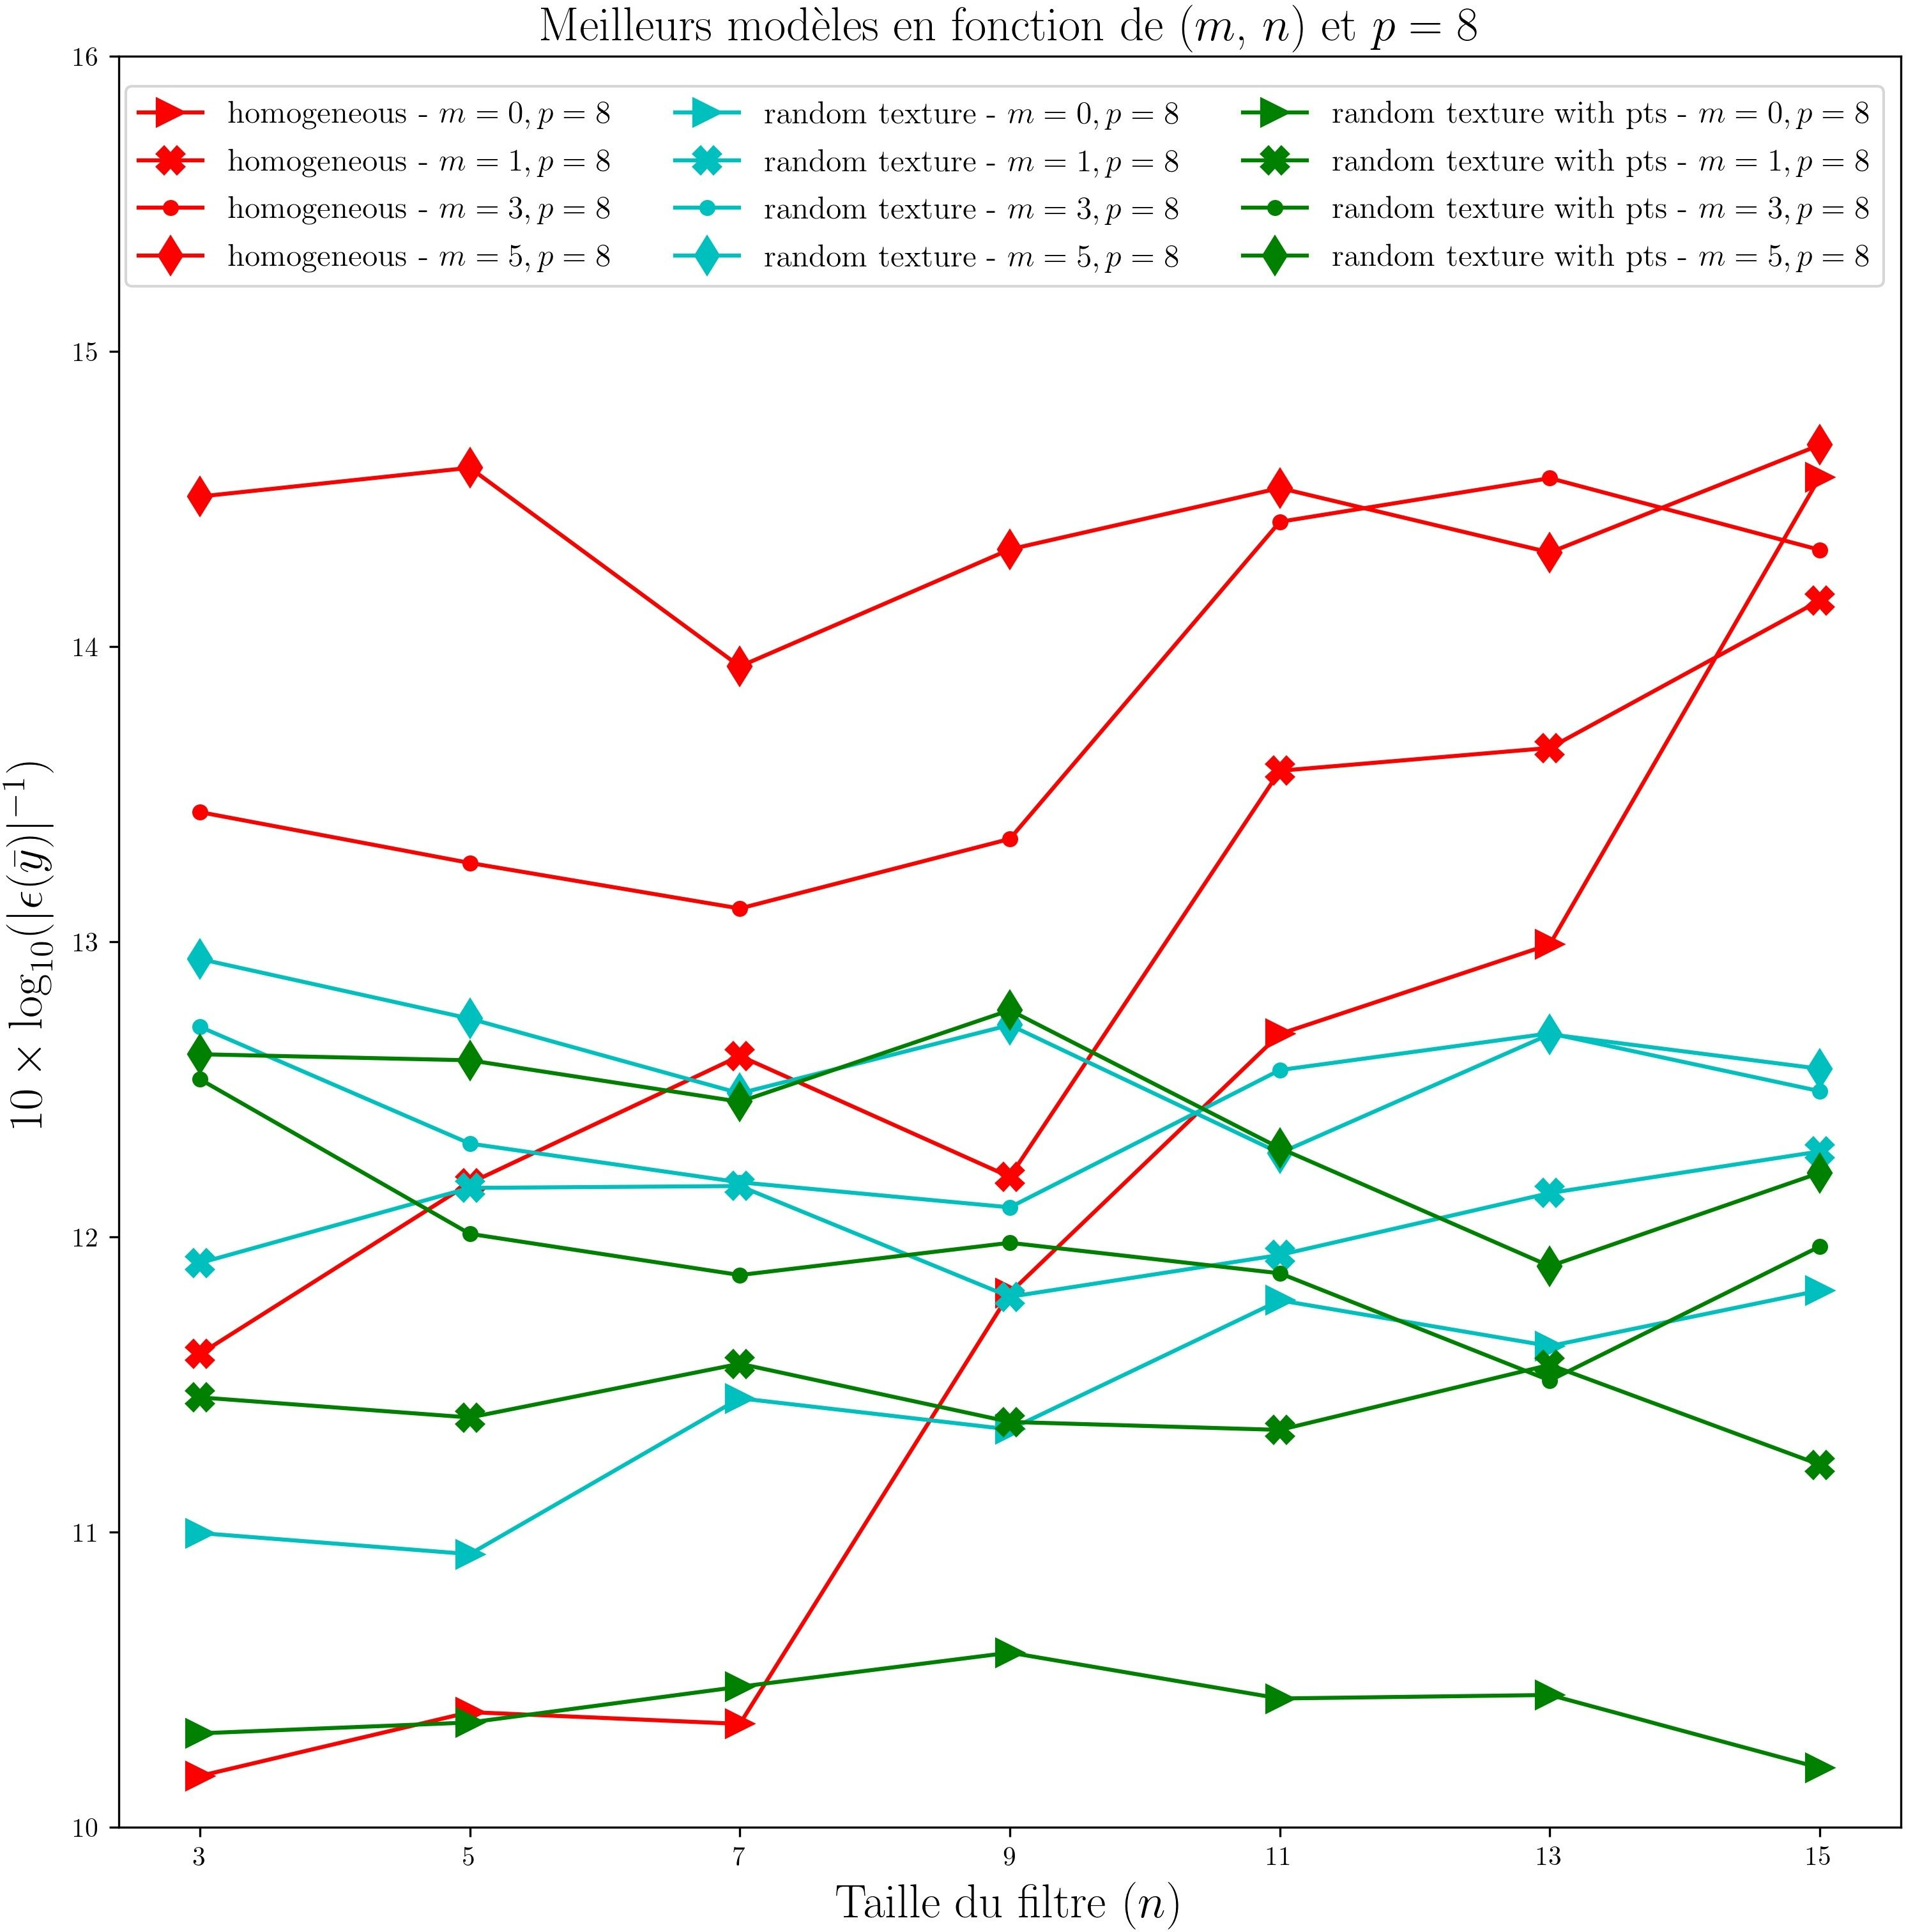
\includegraphics[width=0.75\textwidth]{figures/Chap4/results/best_curves_m=all_p=8_n=all.jpg}
 \centering
  \caption{
  \small{L'erreur de l'apprentissage des meilleurs modèles sur l'ensemble de validation pour les trois expériences: homogène (\textcolor{red}{rouge}), hétérogène (\textcolor{cyan}{cyan}) et hétérogène avec inclusion de cibles ponctuelles (\textcolor{green}{vert}) }
  }
  \label{fig:best_curves_m=all_p=8_n=all}
\end{figure}

La Figure \ref{fig:best_curves_m=all_p=8_n=all} présente les pointages des modèles ayant obtenu les meilleurs performances pour chacun des apprentissages. Les 4 courbes en rouge présentent les performances calculées sur les données d'entraînement homogènes. On observe que pour ces modèles la performance s'améliore à la fois en fonction de la taille $n$ de la couche d'entrée et du nombre $m$ de blocs convolutifs. Les 4 courbes de couleur cyan présentent les performances calculées sur les données d'entraînement hétérogènes. La performance est dégradée et semble n'être sensible qu'au nombre $m$ de blocs convolutifs. La taille $n$ n'améliore que légèrement les résultats que pour la valeur de $m$ égale à 0. Les 4 courbes vertes présentent les performances calculées sur les données d'entraînement hétérogènes avec inclusion de cibles ponctuelles. Les résultats sont légèrement dégradés comparativement aux résultats hétérogènes. La taille $n$ de la couche d'entrée ne semble pas avoir d'influence sur la performance et semble même dégrader les résultats pour les grandes tailles de $n$.

Nous concluons cette section avec la Figure \ref{fig:training_batches} qui présente 16 exemples sortis de l'ensemble de validation ayant servi aux différents apprentissages. Pour les trois ensembles nous montrons:

\begin{enumerate}
    \item L'image caractéristique simulée avec un chatoiement une vue qui constitue la donnée à filtrer;
    \item L'image étiquette qui est la signature unique ou l'ensemble des signatures à cibler selon le cas;
    \item Un exemple de prédiction obtenu au courant des apprentissages;
    \item Une comparaison avec le filtre \textbf{Boxcar} $5\times5$;
\end{enumerate} 

% \begin{figure}[!htbp] 
% 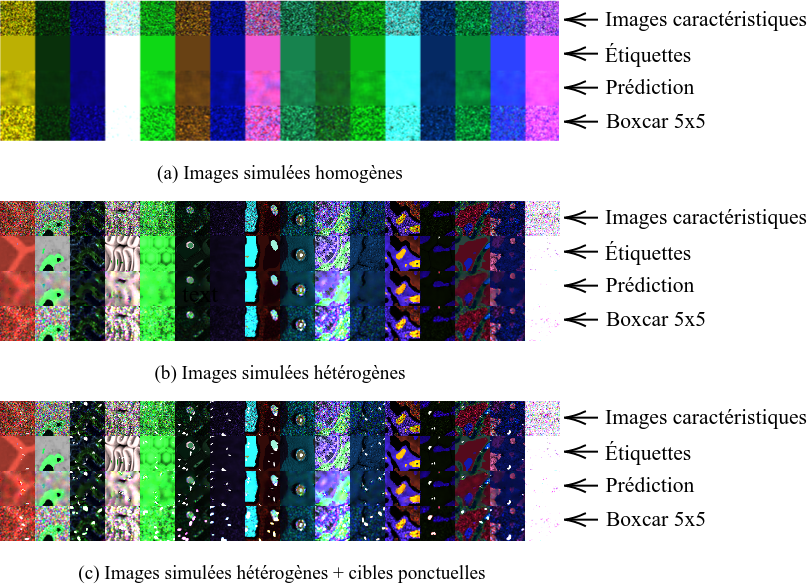
\includegraphics[width=1.0\textwidth]{figures/Chap4/results/training_batches.png}
%  \centering
%   \caption{
%   \scriptsize{Exemple de résultats sur un ensemble de 16 échantillons extrait de l'ensemble de validation. Les trois images présentent en coupe horizontale: 1) le \textit{span} de l'images caractéristiques simulée avec chatoiement $L=1$, 2) le \textit{span} des  étiquettes, 3) le \textit{span} des prédictions et 4) le \textit{span} du filtre boxcar $5 \times 5$}.
%   }
%   \label{fig:training_batches}
% \end{figure}

\begin{figure}[!htbp] 
\centering
\subcaptionbox[]{\scriptsize Imagettes simulées homogènes\label{fig:Imagettes_simulees_homogenes}}
{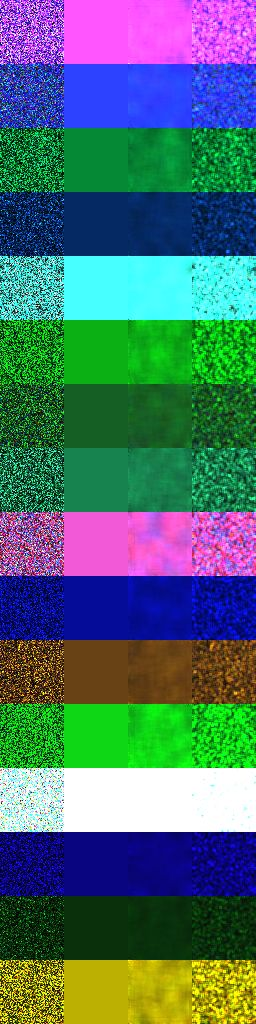
\includegraphics[width=0.3 \textwidth]{figures/Chap4/training_examples_batch/training_homogeneous_batch.jpg}}
\subcaptionbox[]{\scriptsize Imagettes simulées hétérogènes\label{fig:Imagettes_simulees_heterogene}}
{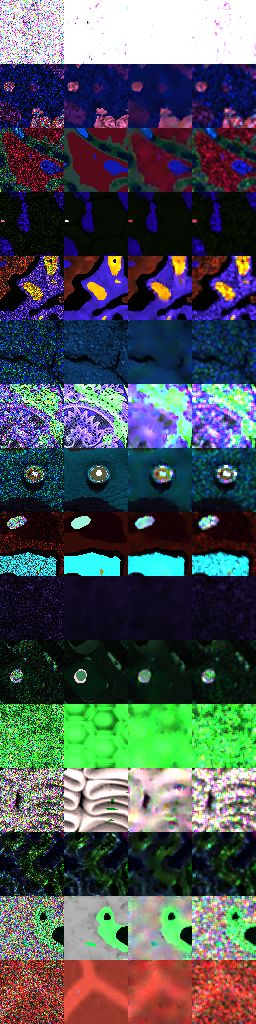
\includegraphics[width=0.3  \textwidth]{figures/Chap4/training_examples_batch/training_random_texture_batch.jpg}}
\subcaptionbox[]{\scriptsize Imagettes simulées hétérogènes + cibles ponctuelles\label{fig:Imagettes_simulees_heterogene_pts}}
{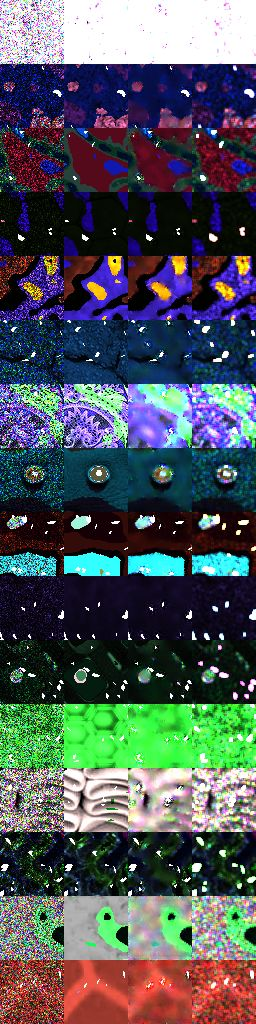
\includegraphics[width=0.3  \textwidth]{figures/Chap4/training_examples_batch/training_random_texture_with_pts_batch.jpg}}
 \caption{
  \small{Exemple de résultats sur un mini-lot de 16 échantillons extraits de l'ensemble de validation. Les trois figures présentent pour chaque type d'apprentissage en colonne: 1) l'image caractéristique simulée avec chatoiement $N=1$, 2) les images étiquettes, 3) les prédictions et 4) le filtre \textbf{Boxcar} $5 \times 5$. $\paulicomposition$}
  }
    \label{fig:training_batches}
\end{figure}

A remarquer que les données pour l'apprentissage des modèles hétérogènes et hétérogènes avec inclusion de cibles ponctuelles sont présentées dans le même ordre car les expériences sont déterministes afin de garantir la reproductibilité des expériences.

\section{L'analyse d'un modèle}

Cette section présente une analyse visuelle des paramètres appris par les réseaux. Nous prenons comme exemple de base le modèle simple à trois couches $m=1$, $p=8$ et $n=15$. Ce modèle est appliqué sur une portion de l'image RADARSAT-2 en matrice de cohérence pour illustrer notre analyse.  

\subsection{Les sorties des couches d'activation}

La technique de visualisation la plus simple est de montrer les activations du réseau pendant la passe en avant. La Figure \ref{fig:activation_viz} montre chacune des activations pour toutes les sorties. La première couche convolutive est représentée sur la figure par la boîte verte annotée $(b)$. Cette couche est formée de 8 convolutions de taille $15\times15$ et les cartes d'activation sont les 8 images respectives associées aux filtres à l'intérieur de la boîte de la figure.  Ces cartes servent par la suite d'intrant à la couche suivante $(c)$ composée aussi de 8 convolutions mais de taille $3\times3$. Elle produisent à leur tour les cartes d'activation secondaires. Et finalement la dernière carte présente le résidu $(d)$ qui  additionné à l'image bruitée $(a)$ donne l'image filtrée $(e)$.
Pour les réseaux avec des couches d'activation de type \textbf{ReLU}, les résultats commencent à paraître relativement \textit{blobby} et denses, mais à mesure que l'apprentissage progresse, les activations deviennent généralement plus rares et localisées. Un piège dangereux que l'on peut facilement remarquer avec cette visualisation est que certaines cartes d'activation peuvent être toutes nulles pour de nombreuses entrées. Ceci peut indiquer des filtres morts et ou bien un symptôme de sur-apprentissage.

\begin{figure}[!htbp] 
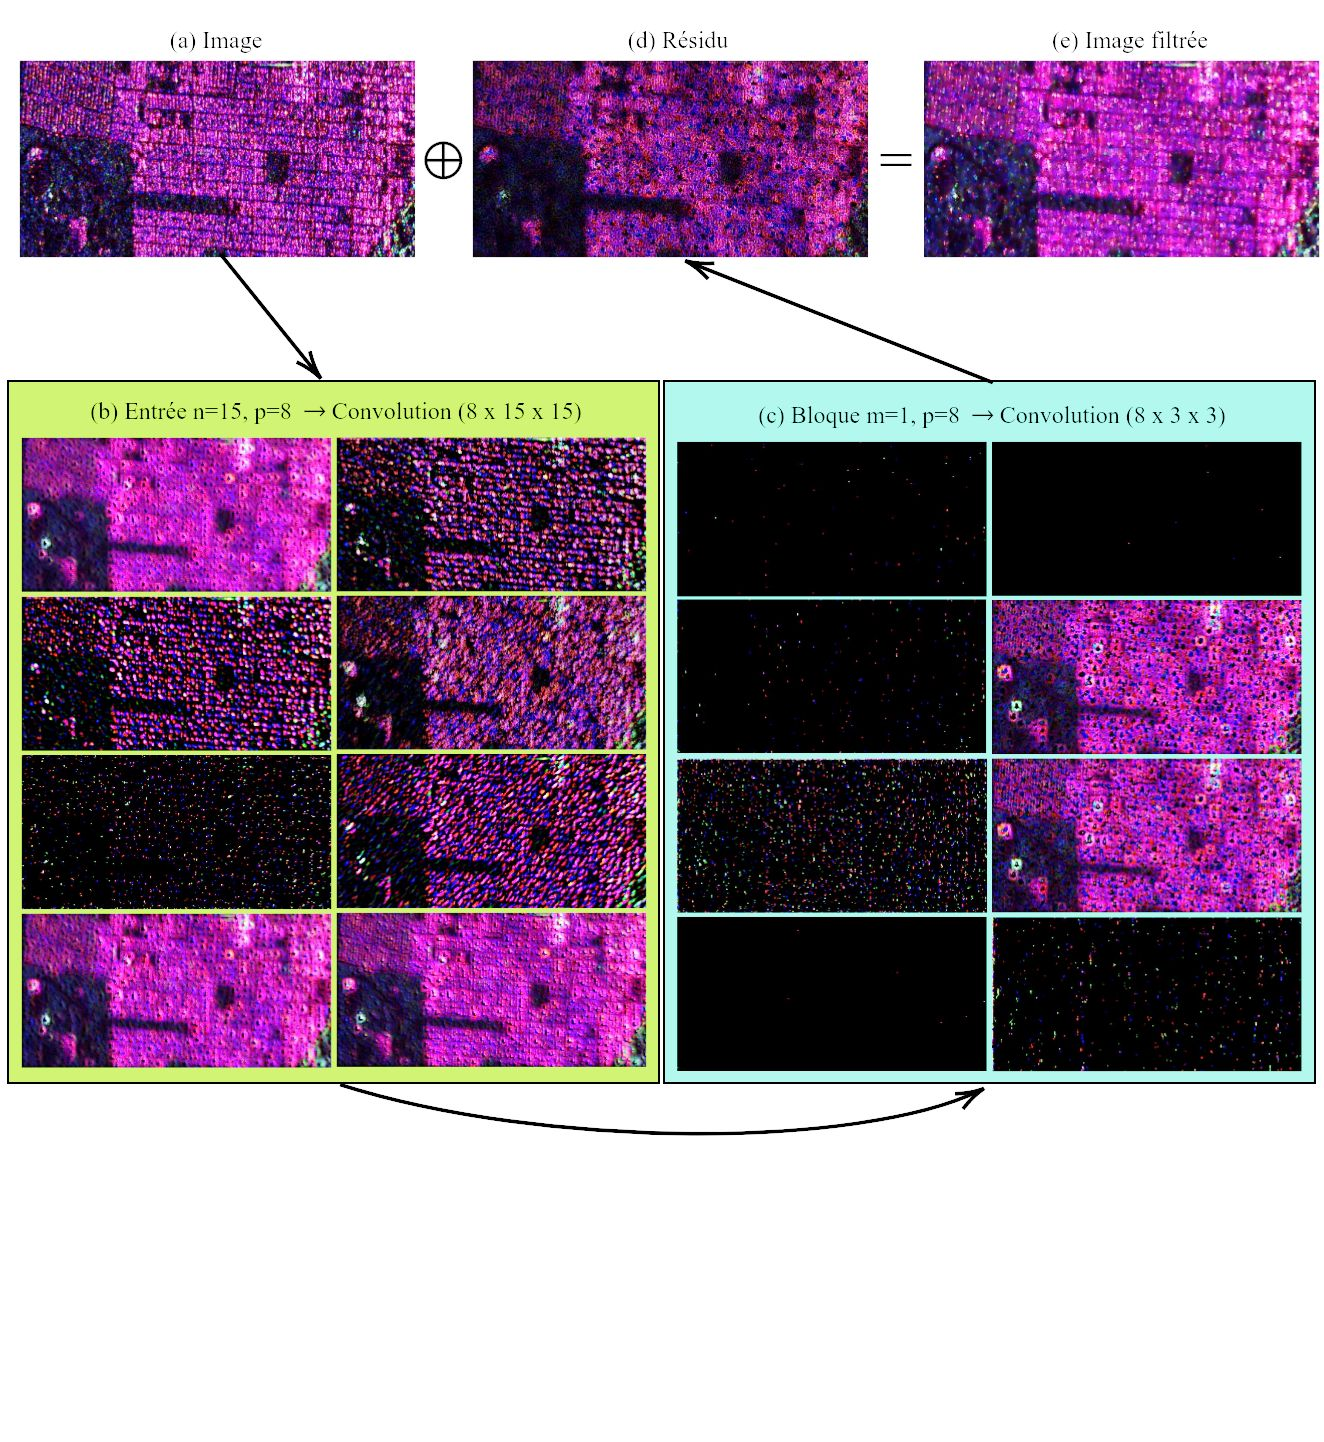
\includegraphics[width=1.1\textwidth]{figures/Chap4/results/analyse_model/activation/activation_viz.jpg}
 \centering
  \caption{
  \small{Exemple des activations du réseau à trois couche $m=1$ $p=8$ $n=15$. La Figure (a) est l'image d'entrée des matrices de cohérence visualisée par le \textit{span}. La Figure (b) montre les 8 activations de la première couche. La Figure (c) montre les 8 activations du bloc convolutif. La Figure (d) présente la carte des résidus et la Figure (e) montre le résultat de l'opération résiduel $\oplus$, $\paulicomposition$.
  }}
  \label{fig:activation_viz}
\end{figure}

\subsection{Les poids des filtres des convolutions}

La deuxième stratégie communément utilisée consiste à visualiser les poids des filtres. Les filtres de la première couche convolutive qui traite directement les données d'entrée sont généralement plus faciles à interpréter et la visualisation de ceux-ci permet de vérifier si le réseau est bien entraîné. Un réseau bien entraîné montre généralement des filtres lisses sans aucun motif bruyant ou aléatoire. Des schémas bruyants peuvent être un indicateur d'un réseau qui n'a pas été entraîné assez longtemps, ou peut-être d'une régularisation insuffisante qui peut avoir conduit à un sur-apprentissage. La Figure \ref{fig:filter_viz}-b donne une représentation intéressante des 8 filtres de taille $15\times15$ de notre réseau exemple. Leur fonction principale est d'extraire des primitives de base comme des lignes ou des points.  Et comme observé par de nombreux travaux en apprentissage machine profond, les filtres de la première couche s'approchent naturellement de la représentation des filtres de Gabor. La représentation en trois dimensions permet de mieux interpréter la fonction des filtres si nous la comparons à la représentation 2-D en intensité (Fig. \ref{fig:filter_viz}-a). L'appréciation générale est bonne et l'on peut discerner que les filtres sont plutôt du type passe-hauts. Les filtres numérotés (7,1) et (2,1) sont de bons exemples de filtres de détection d'arêtes selon une orientation donnée. 
\begin{figure}[!htbp] 
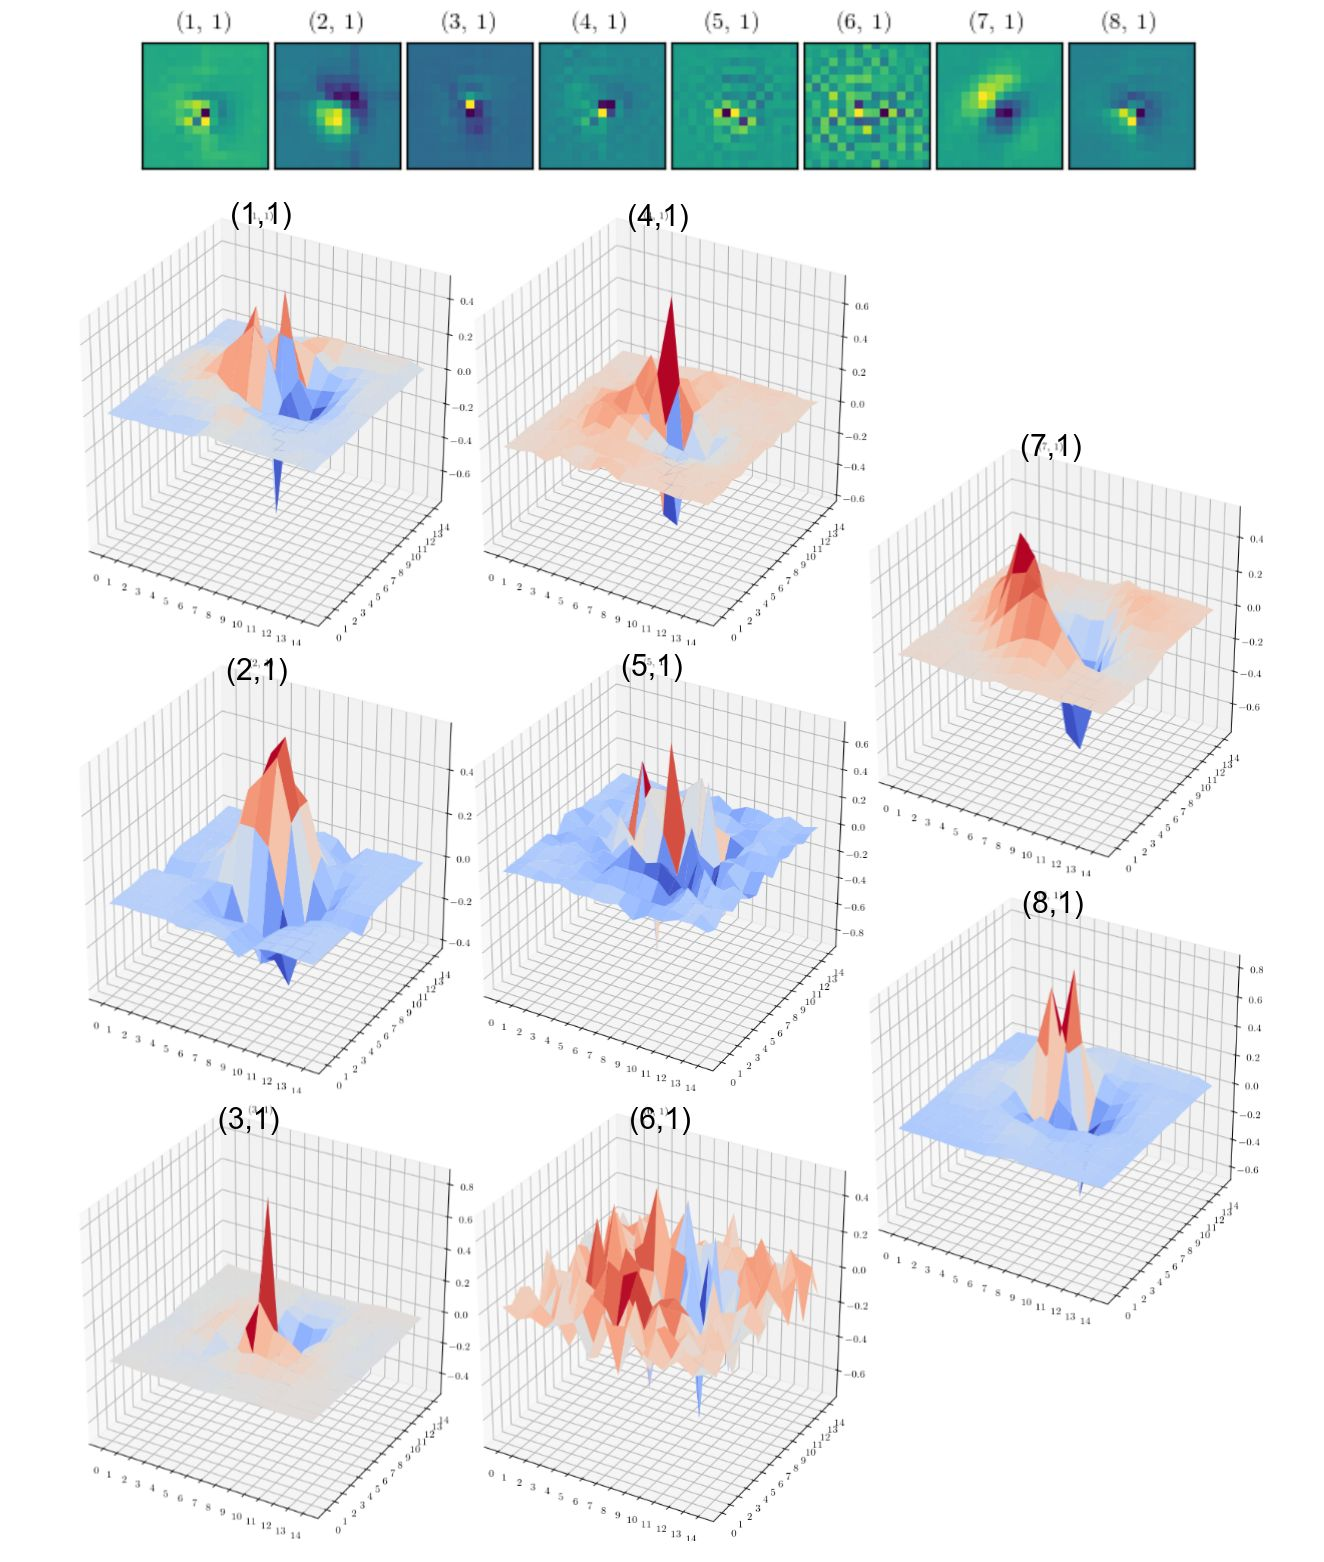
\includegraphics[width=1.1\textwidth]{figures/Chap4/results/analyse_model/activation/filter_viz.jpg}
 \centering
  \caption{
  \small{ Visualisation des filtres $15 \times 15$ de la première couche convolutive.
  }}
  \label{fig:filter_viz}
\end{figure}

%\trainfigall{Apprentissage avec les données simulées homogènes}{homogeneous}{0}
%\trainfigall{Apprentissage avec les données simulées hétérogènes}{random_texture}{0}
%\trainfigall{Apprentissage avec les données simulées hétérogènes avec l'inclusion de cibles ponctuelles}{random_texture_with_pts}{0}


%\trainbestfig{Apprentissage avec les données simulées homogènes}{homogeneous}{0}
%\trainbestfig{Apprentissage avec les données simulées hétérogènes}{random_texture}{0}
%\trainbestfig{Apprentissage avec les données simulées hétérogènes avec l'inclusion de cibles ponctuelles}{random_texture_with_pts}{0}

\section{L'estimation des paramètres de la matrice de cohérence sur les échantillons homogènes } \label{section:estimation_cohérence_homogene}

Cette section présente les résultats de l'estimation des matrice de cohérence pour certaines des classes de diffuseurs polarimétriques de la décomposition \halpha. À la Section \ref{sec:simulation_de_region_homomgene} nous avons décrit le procédé par lequel nos simulations de signatures sur des surfaces homogènes de tailles $256 \times 256$ ont été produites à partir des matrices de cohérences du tableau \ref{tab:sanfrancisco-coherence matrices}. Ces échantillons ont été filtrés par les modèles produits sur les données d'entraînement homogènes. À titre de comparaison, nous avons appliqué les filtres "standard" polarimétriques suivants aux échantillons:

\begin{enumerate}
    \item Le filtre de la moyenne (\textbf{Boxcar});
    \item Le filtre de Lee affiné (\textbf{Refined Lee});
    \item Le filtre de Lee Sigma (\textbf{Sigma Lee});
    \item Le filtre \textbf{IDAN};
\end{enumerate}

Nous présentons les résultats pour les trois grandes classes de diffuseurs selon les angles $\bar{\alpha}$ du diagramme \halpha suivants:

\begin{enumerate}
    \item Les diffuseurs de type \textbf{double bond} représentés par la classe \textbf{Z4} (\textbf{Double réflection}); 
    \item Les diffuseurs de type \textbf{volumétrique} représentés par la la classe \textbf{Z5} (\textbf{Particules anisotropiques}); 
    \item Les diffuseurs de type \textbf{surfacique} représentés par la la classe \textbf{Z3} (\textbf{Surfaces de Bragg}); 
\end{enumerate}

La plupart des résultats sont présentés sous la forme de graphiques qui illustrent l'estimé d'un paramètre polarimétrique en fonction de la taille $n$ de la fenêtre d'entrée et de l'algorithme utilisé pour filtrer les imagettes. Chaque courbe des graphiques correspond à un filtre en particulier et est identifiée avec une ligne de couleur unique. Un marqueur identifie tous les types de filtres. Les filtres que nous avons entraînés portent le même marqueur $\triangle$ mais de couleur différente. La Figure \ref{fig:legend_fig} montre la légende qui sera affichée sur chaque graphique pour départager les résultats.

\begin{figure}[!htbp] 
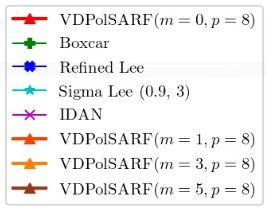
\includegraphics[width=0.33\textwidth]{figures/Chap4/results/legende.jpg}
 \centering
  \caption{
  \small{Exemple de la légende utilisée pour identifier les différents algorithmes de filtrage.
  }}
  \label{fig:legend_fig}
\end{figure}

Les Figures \ref{fig:C_avg_t3_homogeneous_homogeneous_Double_Reflection}, \ref{fig:C_avg_t3_homogeneous_homogeneous_Anisotropic_Particles}, \ref{fig:C_avg_t3_homogeneous_homogeneous_Bragg_Surface} montrent les résultats réalisés sur les données homogènes en appliquant les modèles entraînés sur les données d'apprentissage homogènes. Elles présentent la moyenne de l'erreur relative des 9 éléments de la matrices de cohérence pour chacun de nos diffuseurs. Les Figures \ref{fig:C_std_t3_homogeneous_homogeneous_Double_Reflection}, \ref{fig:C_std_t3_homogeneous_homogeneous_Anisotropic_Particles}, \ref{fig:C_std_t3_homogeneous_homogeneous_Bragg_Surface} présentent l'écart-type sur la mesures des moyennes.  

Les figures se séparent en deux parties. La première colonne montre la moyenne des erreurs calculées sur les termes diagonaux en puissance ($T11, T22, T33$). Les deux colonnes suivantes donnent les résultats respectifs pour les parties réels et imaginaire des termes croisés ($T12, T13, T23$) de la matrice de cohérence.  Par exemple, pour la valeur $T11$ du \textbf{Boxcar} de taille $n=5$ l'erreur relative $|\epsilon|$ est égale à $15.2 \pm 12.4 \%$ pour la donnée de type \textit{double bond}. Nous remarquons les grandes amplitudes au niveau de certains termes croisés. Ces derniers peuvent diverger de plus de 400 \%. Ceci s'explique par le fait que les valeurs sont extrêmement petites et proches de zéro mais non-nulle. Un petit changement est susceptible de générer une grande erreur relative à cause de la petite valeur au dénominateur du calcul. Il est à noter que nous avons expressément généré des matrices de cohérence telles qu'aucun élément de la matrice est nul afin d'éviter le piège de la division par zéro.

Le filtre \textbf{Boxcar} sépare les résultats en deux ensembles en fonction des filtres. Les filtres "standards" obtiennent généralement des résultats inférieurs au \textbf{Boxcar}. Le filtre \textbf{IDAN} présente des résultats plus biaisés par rapport aux termes en puissance si on le compare aux autres filtres. Il atteint rapidement une asymptote de l'ordre de 23 \% indépendamment du nombre de pixels utilisés pour effectuer ses estimés. Par contre il donne souvent de meilleurs résultats pour le terme $im\{T13\}$ que les autres filtres "standard". L'explication valable vient que l'estimé par la médiane est moins biaisé sur la distribution presque symétrique des partie réelles et imaginaires des termes croisés comparée à l'estimation calculées sur les distributions non-symétriques des termes diagonaux de la matrice de cohérence. De manière générale le filtre \textbf{Refined LEE} donne des résultats égaux ou légèrement supérieurs au filtre \textbf{Sigma Lee}. Ceci est un peut étonnant compte-tenu du fait que le filtre \textbf{Refined LEE} génère une forme de texture dans les images filtrées tandis que le filtre \textbf{Sigma Lee} semble donner des résultats plus homogènes (Figs.  \ref{fig:filter_comparison_signature_Double_Reflection_partie_2},  \ref{fig:filter_comparison_signature_Anisotropic_Particles_partie_2}, et  \ref{fig:filter_comparison_signature_Bragg_Surface_partie_2} pour une comparaison visuelle).

Les filtres que nous avons entraînés (\textbf{VDPolSARF}) ont des résultats supérieurs comparés aux filtres "standards". Ils ont une asymptote qui tend vers un biais égal ou meilleur que le filtre \textbf{Boxcar} avec une large fenêtre ($n=15$). On remarque que les résultats tendent à devenir indépendants de la taille de la fenêtre d'entrée lorsque le nombre de couches augmentent. Le filtre \textbf{VDPolSARF} ($m=0, p=8, n=3$) qui ne contient que deux couches se comporte comme un filtre \textbf{Boxcar} mais amélioré. Par exemple pour l'estimé $T11$ du diffuseur volumétrique (Fig. \ref{fig:C_avg_t3_homogeneous_homogeneous_Anisotropic_Particles} et Fig.  \ref{fig:C_std_t3_homogeneous_homogeneous_Anisotropic_Particles}), le \textbf{Boxcar} tend vers un biais de $5.0 \pm 3.7 \% $ et pour notre filtre le biais tend vers $4.9 \pm 3.7 \%$. Tous deux ont des biais et des écart-types qui décroissent en fonction de la taille de l'échantillon.  Le biais de départ ($n=3$) pour le filtre \textbf{Boxcar} est de $26.2 \pm 20.4 \%$ et pour notre filtre nous obtenons un biais de $15.7 \pm 11.9 \%$. Pour le filtre \textbf{VDPolSARF}, l'amélioration du biais et de son écart-type en fonction du nombre de blocs convolutifs ($m$) est intéressante car elle permet à première vue d'éliminer la variable de la taille de la fenêtre d'entrée.  Les biais et leur écart-types décroissent de $29 \%$ de $m=0$ ($15.7 \pm 11.9 \%$) à $m=1$ ($11.1 \pm 8.4 \%$), de $36 \%$ de $m=1$ à $m=3$ ($7.0 \pm 5.3 \%$) et de $25 \%$ de $m=3$ à $m=5$ ($5.3 \pm 3.9 \%$).  Au total entre $m=0$ et $m=5$ nous avons une amélioration du biais de l'ordre de 66 \% en empilant 5 couches de blocs convolutifs avec des filtres $3 \times 3$.

Nous remarquons que l'estimation semble meilleure sur les termes en puissance de la matrice de cohérence et ceci pour chaque diffuseur.  Les termes complexes sont plus variables et semblent plus difficiles à estimer pour les filtres courts ($m=0,1$). Nous avons de moins bons résultats pour les tailles de fenêtres $n=9$ et $n=15$. Ils sortent de la courbe attendue: monotone et décroissante.  Est-ce un effet du hasard de l'apprentissage? La question demeure ouverte mais l'apprentissage des filtres plus courts semble être plus imprécis pour les grandes tailles de fenêtre.  

En conclusion de cette section nous pouvons considérer que les filtres appris sont de bons estimateurs de la matrice de cohérence pour les données une vue sur les surfaces homogènes. En particulier la famille des filtres plus profond $m=3,  5, p=8$ donnent les meilleurs performances en terme de biais.  Les biais et leurs écart-types demeurent constants en fonction de la taille de la fenêtre. 

\matcohfigavgallC{all}{8}{0}{homogeneous}{simulated_signatures_T3}{Double_Reflection}{Diffuseurs}{double bond}{homogeneous}  
\matcohfigstdevallC{all}{8}{0}{homogeneous}{simulated_signatures_T3}{Double_Reflection}{Diffuseurs}{double bond}{homogeneous} 

\matcohfigavgallC{all}{8}{0}{homogeneous}{simulated_signatures_T3}{Anisotropic_Particles}{Diffuseurs}{volumétriques}{homogeneous} 
\matcohfigstdevallC{all}{8}{0}{homogeneous}{simulated_signatures_T3}{Anisotropic_Particles}{Diffuseurs}{volumétriques}{homogeneous} 

\matcohfigavgallC{all}{8}{0}{homogeneous}{simulated_signatures_T3}{Bragg_Surface}{Diffuseurs}{surfaciques}{homogeneous}
\matcohfigstdevallC{all}{8}{0}{homogeneous}{simulated_signatures_T3}{Bragg_Surface}{Diffuseurs}{surfaciques}{homogeneous} 

\section{L'estimation du nombre de vue équivalent sur les échantillons homogènes}

Cette section présente les résultats sur l'estimation du nombre équivalent de vues (\textbf{NEV}) sur les échantillons homogènes de nos trois diffuseurs.  Cette mesure indique l’intensité de réduction du chatoiement et nous la calculons sur les trois termes en puissance ($T11, T22, T33$) de la matrice de cohérence.  Nous rappelons que les échantillons non filtrés ont un $\textbf{NEV} \approx 1$ (voir Tab.  \ref{tab:homogeneous_enl_table}).  Sur les images en intensité, le \textbf{NEV} est calculé comme suit:

\begin{equation}
    NEV = \frac{1}{  \beta^2}
\end{equation}

où $\beta$ est défini comme le ratio de l'écart-type sur la moyenne des intensités $I$:

\begin{equation}
\beta=\frac{\sqrt{E\left[(I-E\left[I\right])\right]^2}}{E\left[I\right]}
\end{equation}

Les Figures \ref{fig:enl_Double_Reflection}, \ref{fig:enl_Anisotropic_Particles} et \ref{fig:enl_Bragg_Surface} présentent le calcul du \textbf{NEV} pour chacun des filtres appliqués aux échantillons homogènes de nos trois types de diffuseurs. Les différentes courbes illustrent le \textbf{NEV} en fonction de la taille $n$ de la fenêtre utilisée pour filtrer les données polarimétriques. La courbe du filtre \textbf{Boxcar} sépare les résultats en deux groupes.  Les filtres "standards" présentent une réduction du chatoiement plus faible que le \textbf{Boxcar}.   Le filtre \textbf{IDAN} ne semble pas aussi efficace pour la réduction du chatoiement que les autres filtres. Les \textbf{NEV} demeurent faibles peu importe la taille en pixels utilisés pour faire les calculs.  Le filtre \textbf{Refined LEE} donne de meilleurs résultats en fonction de la taille de la fenêtre que son homologue \textbf{Sigma Lee}. Le \textbf{NEV} du filtre \textbf{Refined LEE} semble croître de manière exponentielle comme le \textbf{Boxcar} tandis que le filtre \textbf{Sigma Lee} semble croitre de manière logarithmique et tend à plafonner en fonction de la taille de la fenêtre.  Le tableau \ref{tab:refine_lee_nev} donne les valeurs maximales du \textbf{NEV} calculés sur les termes diagonaux des diffuseurs pour le filtre \textbf{Refined LEE} ($11 \times 11$) et du filtre \textbf{Boxcar} de même taille. Grossièrement le \textbf{NEV} du filtrage par \acrconvnet est doublé par rapport à celui du le filtre \textbf{Boxcar} .

\begin{table}[!htbp]
\centering
\begin{tabular}{|l|l|l|l|}
\hline
                     & \textbf{T11} & \textbf{T22} & \textbf{T33}                       \\ \hline
\textbf{Diffuseurs double bond} & 81.3 / 119.8      & 66.8 / 110.3        & 65.2 / 115.4           \\ \hline 
\textbf{Diffuseurs volumétriques}      & 61.7  / 135.2         & 61.4  / 117.1       & 58.5 / 119.7       \\ \hline
\textbf{Diffuseurs surfaciques}     & 69.6 / 119.8        & 68.8 / 122.9        & 67.2 / 117.0         \\ \hline  
\end{tabular}
\caption{\small{Les nombres équivalents de vue calculés sur les échantillons des trois diffuseurs typiques filtrés par le filtre \textbf{Refined LEE} ($n=11$) comparées aux valeurs du filtre \textbf{Boxcar} ($n=11$).  Les \textbf{NEV} sont calculés sur les termes en puissance de la matrice de cohérence. }
}
\label{tab:refine_lee_nev}
\end{table}

Dans le cas des filtres appris, la performance est soit égale ou nettement supérieure au \textbf{Boxcar}. La famille des filtres les plus courts ($m=0$, $p=8$) se comporte sensiblement comme ce dernier en fonction de la taille de la fenêtre. Tandis que les filtres les plus profonds ($m=5$, $p=8$) montrent des performances supérieures de plusieurs ordres de magnitude pour des petites tailles de fenêtres comparés au \textbf{Boxcar} (voir tab \ref{tab:vdpolsarf_lee_nev}).  Comme nous l'avons remarqué à la section \ref{section:estimation_cohérence_homogene}, les filtres \textbf{VDPolSARF} profonds sont moins sensibles à la taille $n$ de la fenêtre d'entrée pour l'estimation de la matrice de cohérence.  Par contre dans le cas du calcul du \textbf{NEV}, la taille du filtre a une influence marquée sur le calcul de celui-ci et ceci pour tous les diffuseurs.  Le tableau \ref{tab:vdpolsarf_lee_nev} met en relief la différence entre les filtres \textbf{VDPolSARF} et \textbf{Boxcar} de taille $n=11$.  La réduction du chatoiement est approximativement triplée en faveur du premier. Nous remarquons que pour les filtres de la famille ($m=3, p=8$), l'augmentation de la performance s'arrête après le point culminant à $n=11$.  Nous sommes sans explications par rapport à cette observation.


\begin{table}[!htbp]
\centering
\begin{tabular}{|l|l|l|l|}
\hline
                     & \textbf{T11} & \textbf{T22} & \textbf{T33} \\ \hline
\textbf{Diffuseurs double bond} & 306.7 / 119.8      & 258.2 / 110.3        & 272.6 / 115.4        \\ \hline 
\textbf{Diffuseurs volumétriques}      & 347.6  / 135.2         & 281.9  / 117.1       & 300.8 / 119.7        \\ \hline
\textbf{Diffuseurs surfaciques}     & 289.7 / 119.8        & 299.0 / 122.9        & 272.8 / 117.0     \\ \hline  
\end{tabular}
\caption{\small{Les nombres équivalents de vue calculés sur les échantillons des trois diffuseurs typiques filtrés par le filtre de \textbf{VDPolSARF} ($m=5, p=8, n=11$) comparées aux valeurs du filtre \textbf{Boxcar} de même taille.  Les \textbf{NEV} sont calculés sur les termes en puissance de la matrice de cohérence. }
}
\label{tab:vdpolsarf_lee_nev}
\end{table}

Pour conclure cette section nous présentons un aperçu visuel des résultats du filtrage. Les figures sont présentées en deux parties par diffuseur. Les Figures \ref{fig:filter_comparison_signature_Double_Reflection_partie_1} et \ref{fig:filter_comparison_signature_Double_Reflection_partie_2} montrent les résultats des filtrages sur le diffuseur \textit{double bond}, les Figures \ref{fig:filter_comparison_signature_Anisotropic_Particles_partie_1} et  \ref{fig:filter_comparison_signature_Anisotropic_Particles_partie_2} montrent les résultats des filtrages sur le diffuseur volumétrique, et finalement les Figures \ref{fig:filter_comparison_signature_Bragg_Surface_partie_1} et \ref{fig:filter_comparison_signature_Bragg_Surface_partie_2} montrent les résultats des filtrages sur le diffuseur surfacique.  Dans la première partie de chaque paire des figures et sur la première ligne nous affichons l'image caractéristique et l'image étiquette associée au diffuseur.  Ensuite, les filtrages pour les deux tailles de fenêtres $n=5$ et $n=13$ du filtre \textbf{VDPolSARF} et \textbf{Boxcar} sont affichés.  Dans la seconde partie nous continuons l'affichage du filtrage obtenu à partir du filtre \textbf{Refined LEE}, du filtre \textbf{Sigma Lee} et du filtre \textbf{IDAN}. Toutes les images présentent les valeurs du \textit{span} selon l'ordre  $\paulicomposition$: ce qui correspond aux termes de la matrice de cohérence (T22, T33, T11).  La visualisation met particulièrement en valeur le lissage soutenu du filtre \textbf{VDPolSARF} pour les deux tailles de filtres  $n=5$ et $n=13$.


\enlfigures{Double_Reflection}{Diffuseurs}{double bond}{homogeneous}{entraînés sur les données d'apprentissage homogènes}

\enlfigures{Anisotropic_Particles}{Diffuseurs}{volumétriques}{homogeneous}{entraînés sur les données d'apprentissage homogènes}

\enlfigures{Bragg_Surface}{Diffuseurs}{surfaciques}{homogeneous}{entraînés sur les données d'apprentissage homogènes}

\homegeneousresults{signature_Double_Reflection}{Diffuseurs}{double bond}{entraînés sur les données d'apprentissage homogènes}
\homegeneousresults{signature_Anisotropic_Particles}{Diffuseurs}{volumétriques}{entraînés sur les données d'apprentissage homogènes}
\homegeneousresults{signature_Bragg_Surface}{Diffuseurs}{surfaciques}{entraînés sur les données d'apprentissage homogènes}

\section{L'estimation des paramètres de la décomposition H-A-Alpha sur les données homogènes}

Cette section présente les résultats relatifs à la décomposition \haalpha des échantillons filtrés pour nos trois diffuseurs types.  Les Figures \ref{fig:C_avg_homogeneous_haalpha_homogeneous_bias_Double_Reflection}, \ref{fig:C_avg_homogeneous_haalpha_homogeneous_bias_Anisotropic_Particles}  et \ref{fig:C_avg_homogeneous_haalpha_homogeneous_bias_Bragg_Surface} montrent la moyenne des erreurs relatives en fonction de la taille $n$ de la fenêtre d'entrée et ceci pour chacun des filtres "standards" et appris. De façon similaire, les Figures \ref{fig:C_std_homogeneous_haalpha_homogeneous_bias_Double_Reflection}, \ref{fig:C_std_homogeneous_haalpha_homogeneous_bias_Anisotropic_Particles}  et \ref{fig:C_std_homogeneous_haalpha_homogeneous_bias_Bragg_Surface} montrent l'écart-type des erreurs relatives en fonction de la taille $n$ de la fenêtre d'entrée et ceci pour chacun de filtres "standards" et appris.  Les graphes présentent les résultats pour chaque terme de la décomposition, soit l'entropie, l'anisotropie et l'angle $\bar{\alpha}$ (voir section \ref{section:decomposition_polarimetric} pour les aspects théoriques).

Dans le cas de l'estimation de l'entropie des diffuseurs de type \textit{double bond} et volumétrique, l'observation générale est que les modèles appris se comportent mieux que les filtres "standards" ou sont similaires au filtre \textbf{Boxcar}.  Par contre pour le diffuseur surfacique, on remarque des erreurs plus élevées et des résultats plus incertains après que la taille $n$ de la première couche convolutive dépasse 7 pour les modèles courts ($m=0, 1$). Cependant pour les modèles profonds ($m=5$) les résultats sont semblables au filtre \textbf{Boxcar} à large fenêtre $15 \times 15$.

\begin{table}[!htbp]
\centering
\begin{tabular}{|l|l|l|l|}
\hline
                     & \textbf{Double bond} & \textbf{Volume} & \textbf{Surface} \\ \hline
\textbf{VDPLSARF} ($m=5, p=8$, $n=15$) & \valuepc{1.7}{1.3}    & \valuepc{1.1}{0.1}      & \valuepc{5.3}{4.1}         \\ \hline 
\textbf{\textbf{Boxcar} $15 \times 15$}      & \valuepc{2.1}{1.6}         & \valuepc{1.4}{0.1}       & \valuepc{4.6}{3.4}           \\ \hline
\end{tabular}
\caption{\small{Biais relatifs sur l'estimé de l'entropie.  Comparaison entre le modèle \textbf{VDPLSARF} ($m=5, p=8$, $n=15$) et le filtre \textbf{Boxcar}  $15 \times 15$}}
\label{tab:vdpolsarf_angle_entropie}
\end{table}

Dans le cas  du diffuseur \textit{double bond}, l'estimation de l'anisotropie est légèrement moins bonne pour les modèles courts ($m=0,1$) ou égale ou supérieure pour les modèles plus profonds ($m=3,5$) si nous les comparons aux résultats du \textbf{Boxcar}.  Dans le cas du diffuseur volumétrique les résultats sont égaux ou supérieurs au \textbf{Boxcar}.  Par contre pour le diffuseur surfacique les résultats sont nettement moins précis pour les modèles courts ($m=0, 1$).

\begin{table}[!htbp]
\centering
\begin{tabular}{|l|l|l|l|}
\hline
                     & \textbf{Double bond} & \textbf{Volume} & \textbf{Surface} \\ \hline
\textbf{VDPLSARF} ($m=5, p=8$, $n=15$) & \valuepc{3.4}{2.7}    & \valuepc{15.7}{11.2}      & \valuepc{19.3}{14.3}         \\ \hline 
\textbf{\textbf{Boxcar} $15 \times 15$}      & \valuepc{4.1}{3.1}         & \valuepc{19.5}{14.4}       & \valuepc{14.8}{11.1}           \\ \hline
\end{tabular}
\caption{\small{Biais relatifs sur l'estimé de l'anisotropie.  Comparaison entre le modèle \textbf{VDPLSARF} ($m=5, p=8$, $n=15$) et le filtre \textbf{Boxcar} $15 \times 15$.}}
\label{tab:vdpolsarf_angle_anisotropie}
\end{table}

Dans le cas du paramètres $\bar{\alpha}$, l'estimation est égale et supérieure au filtre \textbf{Boxcar}. Le biais relatif est semblable pour les trois type de diffuseur (voir Tab.  \ref{tab:vdpolsarf_angle_alpha}).


\begin{table}[!htbp]
\centering
\begin{tabular}{|l|l|l|l|}
\hline
                     & \textbf{Double bond} & \textbf{Volume} & \textbf{Surface} \\ \hline
\textbf{VDPLSARF} ($m=5, p=8$, $n=15$) & \valuepc{1.9}{1.4}    & \valuepc{2.2}{1.7}      & \valuepc{1.7}{1.3}         \\ \hline 
\textbf{\textbf{Boxcar} $15 \times 15$}      & \valuepc{3.3}{1.8}         & \valuepc{2.8}{2.1}       & \valuepc{2.1}{1.5}           \\ \hline
\end{tabular}
\caption{\small{Biais relatifs sur l'estimé de l'angle $\bar{\alpha}$. Comparaison entre le modèle \textbf{VDPLSARF} ($m=5, p=8$, $n=15$) et le filtre \textbf{Boxcar} $15 \times 15$.}}
\label{tab:vdpolsarf_angle_alpha}
\end{table}

En conclusion à cette section, les observations montrent que la précision des paramètres n'est pas garantie pour tous les modèles.  En particulier pour les modèles courts ($m=0,1$) et les grandes fenêtres $n$. Cependant pour le modèle le plus long ($m=5, p=8$) les résultats semblent stables pour l'anisotropie.  

\haalphafigavgallC{all}{8}{0}{homogeneous_haalpha}{simulated_signatures_haalpha}{Double_Reflection}{Diffuseurs}{double bond}{homogeneous}

\haalphafigstdevallC{all}{8}{0}{homogeneous_haalpha}{simulated_signatures_haalpha}{Double_Reflection}{Diffuseurs}{double bond}{homogeneous}

\haalphafigavgallC{all}{8}{0}{homogeneous_haalpha}{simulated_signatures_haalpha}{Anisotropic_Particles}{Diffuseurs}{volumétriques}{homogeneous}

\haalphafigstdevallC{all}{8}{0}{homogeneous_haalpha}{simulated_signatures_haalpha}{Anisotropic_Particles}{Diffuseurs}{volumétriques}{homogeneous}

\haalphafigavgallC{all}{8}{0}{homogeneous_haalpha}{simulated_signatures_haalpha}{Bragg_Surface}{Diffuseurs}{surfaciques}{homogeneous}

\haalphafigstdevallC{all}{8}{0}{homogeneous_haalpha}{simulated_signatures_haalpha}{Bragg_Surface}{Diffuseurs}{surfaciques}{homogeneous}

\section{La qualité de la reconstruction des détails}

Cette section présente les résultats des modèles appliqués sur les images synthétiques hétérogènes (multi-signatures) avec inclusion de cibles ponctuelles. Les cibles sont ajoutées aléatoirement aux images et leurs intensités peuvent varier entre 3db à 10 db selon le cas.  Nous avons produits originalement 10 images selon la procédure exposée à la Section \ref{section:simulation_heterogeneous_regions}. Par contre notre analyse ne portera que sur deux images afin d'éviter la redondance des résultats.

Les modèles entraînés sur les données hétérogènes avec inclusion de cibles ponctuelles sont utilisés pour filtrer nos images.  Les Figures \ref{fig:filter_comparison_image_0_1} et \ref{fig:filter_comparison_image_0_2} montrent les résultats obtenus pour la première image synthétique. La première des figures présente côte-à-côte sur la première ligne du tableau, l'image caractéristique avec le chatoiement une vue et l'image étiquette.  La seconde ligne montre les résultats du filtrage réalisé par les filtres \textbf{VDPOLSAR} ($m=5, p=8$) de taille $n$ égale à 5 et 13.  La seconde figure  montre les résultats comparatifs des filtres \textbf{Boxcar} et \textbf{Sigma Lee}. La même disposition est employée pour la présentation du filtrage de notre second exemple (Fig. \ref{fig:filter_comparison_image_3_1} et \ref{fig:filter_comparison_image_3_2}). 

L'analyse qualitative par l'inspection visuelle des images montre que les images traitées par les filtres appris se comparent favorablement aux images filtrées par le \textbf{Boxcar}. Dans le cas de ce dernier on observe nettement l'effet de la perte de résolution spatiale et de l'étalement de la radiométrie des cibles sur un large voisinage. Pour le filtre \textbf{VDPolSARF}, les contours sont mieux définis et les cibles ponctuelles sont conservées presque entièrement. Dans le cas du filtre $5 \times 5$, les zones homogènes paraissent mieux filtrées par rapport au filtre \textbf{Sigma Lee}. Cependant nous observons que les filtres appris fabriquent des artéfacts autour des cibles.  A la différence des filtres "standards" qui détectent la présence des cibles pour éviter de les filtrer, les filtres appris tentent plutôt de les restituer à partir du signal d'entrée:  il n'y a pas de détection mais une reconstruction. Cette opération s'avère être une opération plus délicate.

\filterresultsmultisigs{000}{0}
\filterresultsmultisigs{003}{3}

Les Figures \ref{fig:filter_psnr_0} et \ref{fig:filter_psnr_3} présentent l'analyse quantitative sur chacune de nos deux images simulées. Premièrement, nous effectuons une comparaison entre l'image caractéristique filtrée et l'image étiquette afin d'évaluer la reconstruction général. Deuxièmement, nous comparons les résultats du filtre d'un Sobel ($3 \times 3$) appliqué à l'image caractéristique filtrée et à l'image étiquette afin d'évaluer la reconstruction des contours.

Nous utilisons les deux mesures suivantes pour l'évaluation de la reconstruction des détails:

\begin{enumerate}
    \item \textbf{PSNR} (\textit{Peak Signal to Noise Ratio}):
    \item \textbf{SIMM} (\textit{Structural Similarity Index Measure}): 
\end{enumerate}

Le \textbf{PSNR} est formulé comme suit:

\begin{equation}
     \textbf{PSNR} = 10 \times log_{10} \bigg( \frac{d^2}{ \textbf{EQM}} \bigg) 
\end{equation}

où \textbf{EQM} est l'erreur quadratique moyenne:

\begin{equation}
    \textbf{EQM} = \frac{1}{mn}\sum_{i=0}^{m-1} \sum_{j=0}^{j-1} \bigg( I_0(i,j) - I_r(i,j) \bigg)^2 
    \label{eq:PSNR}
\end{equation}

et $I_0$ correspond au images caractéristiques avec chatoiement et $I_r$ aux images étiquettes.  Nous avons fixé la valeur $d=3 dB$ et les images ont été seuillées en conséquence.

Le \textbf{SSIM} est formulé comme suit:

\begin{equation}
  SSIM = \frac{(2\mu_x\mu_y + C_1) + (2 \sigma _{xy} + C_2)} 
    {(\mu_x^2 + \mu_y^2+C_1) (\sigma_x^2 + \sigma_y^2+C_2)}
  \label{eq:SSMI}
\end{equation}

où $\mu_x$ est la moyenne de $I_0$ et$\mu_y$ est la moyenne de $I_r$, $\sigma_x^2$ est la variance de $I_0$ et $\sigma_y^2$ est la variance de $I_r$, $C_1$ et $C_2$ sont deux constantes.

Les Figures \ref{fig:filter_psnr_0} et \ref{fig:filter_psnr_3}  présentent les résultats suivants:

\begin{enumerate}
    \item La comparaison des \textbf{PSNR} pour chacun des filtres en fonction de la taille $n$ de l'entrée du filtre par rapport à l'image étiquette;
    \item La comparaison des \textbf{SSIM} pour chacun des filtres en fonction de la taille $n$ de l'entrée du filtre par rapport à l'image étiquette;
    \item La comparaison des \textbf{PSNR} sur les images de Sobel pour chacun des filtres en fonction de la taille $n$ de l'entrée du filtre par rapport à l'image de Sobel étiquette;
    \item La comparaison des \textbf{SSIM} sur les images de Sobel pour chacun des filtres en fonction de la taille $n$ de l'entrée du filtre par rapport à l'image de Sobel étiquette;
\end{enumerate}

Nous remarquons que dans le cas du \textbf{PSNR}, le \textbf{Boxcar} et le filtre \textbf{IDAN} donnent les pires résultats. Ce qui est prévisible pour le \textbf{Boxcar} mais étonnant pour le filtre \textbf{IDAN} dont la performance est encore moindre.  Le filtre \textbf{Refined LEE} performe légèrement mieux que les filtres \textbf{Sigma Lee} et \textbf{VDPolSARF} le plus court. Ce sont les filtres appris les plus profonds qui dominent au niveau de la performance.  Le filtre $\textbf{VDPolSARF}$ ($m=5, p=8$) donne les meilleurs résultats et ceci indépendamment de la taille de la fenêtre.


\begin{figure}[!htbp] 
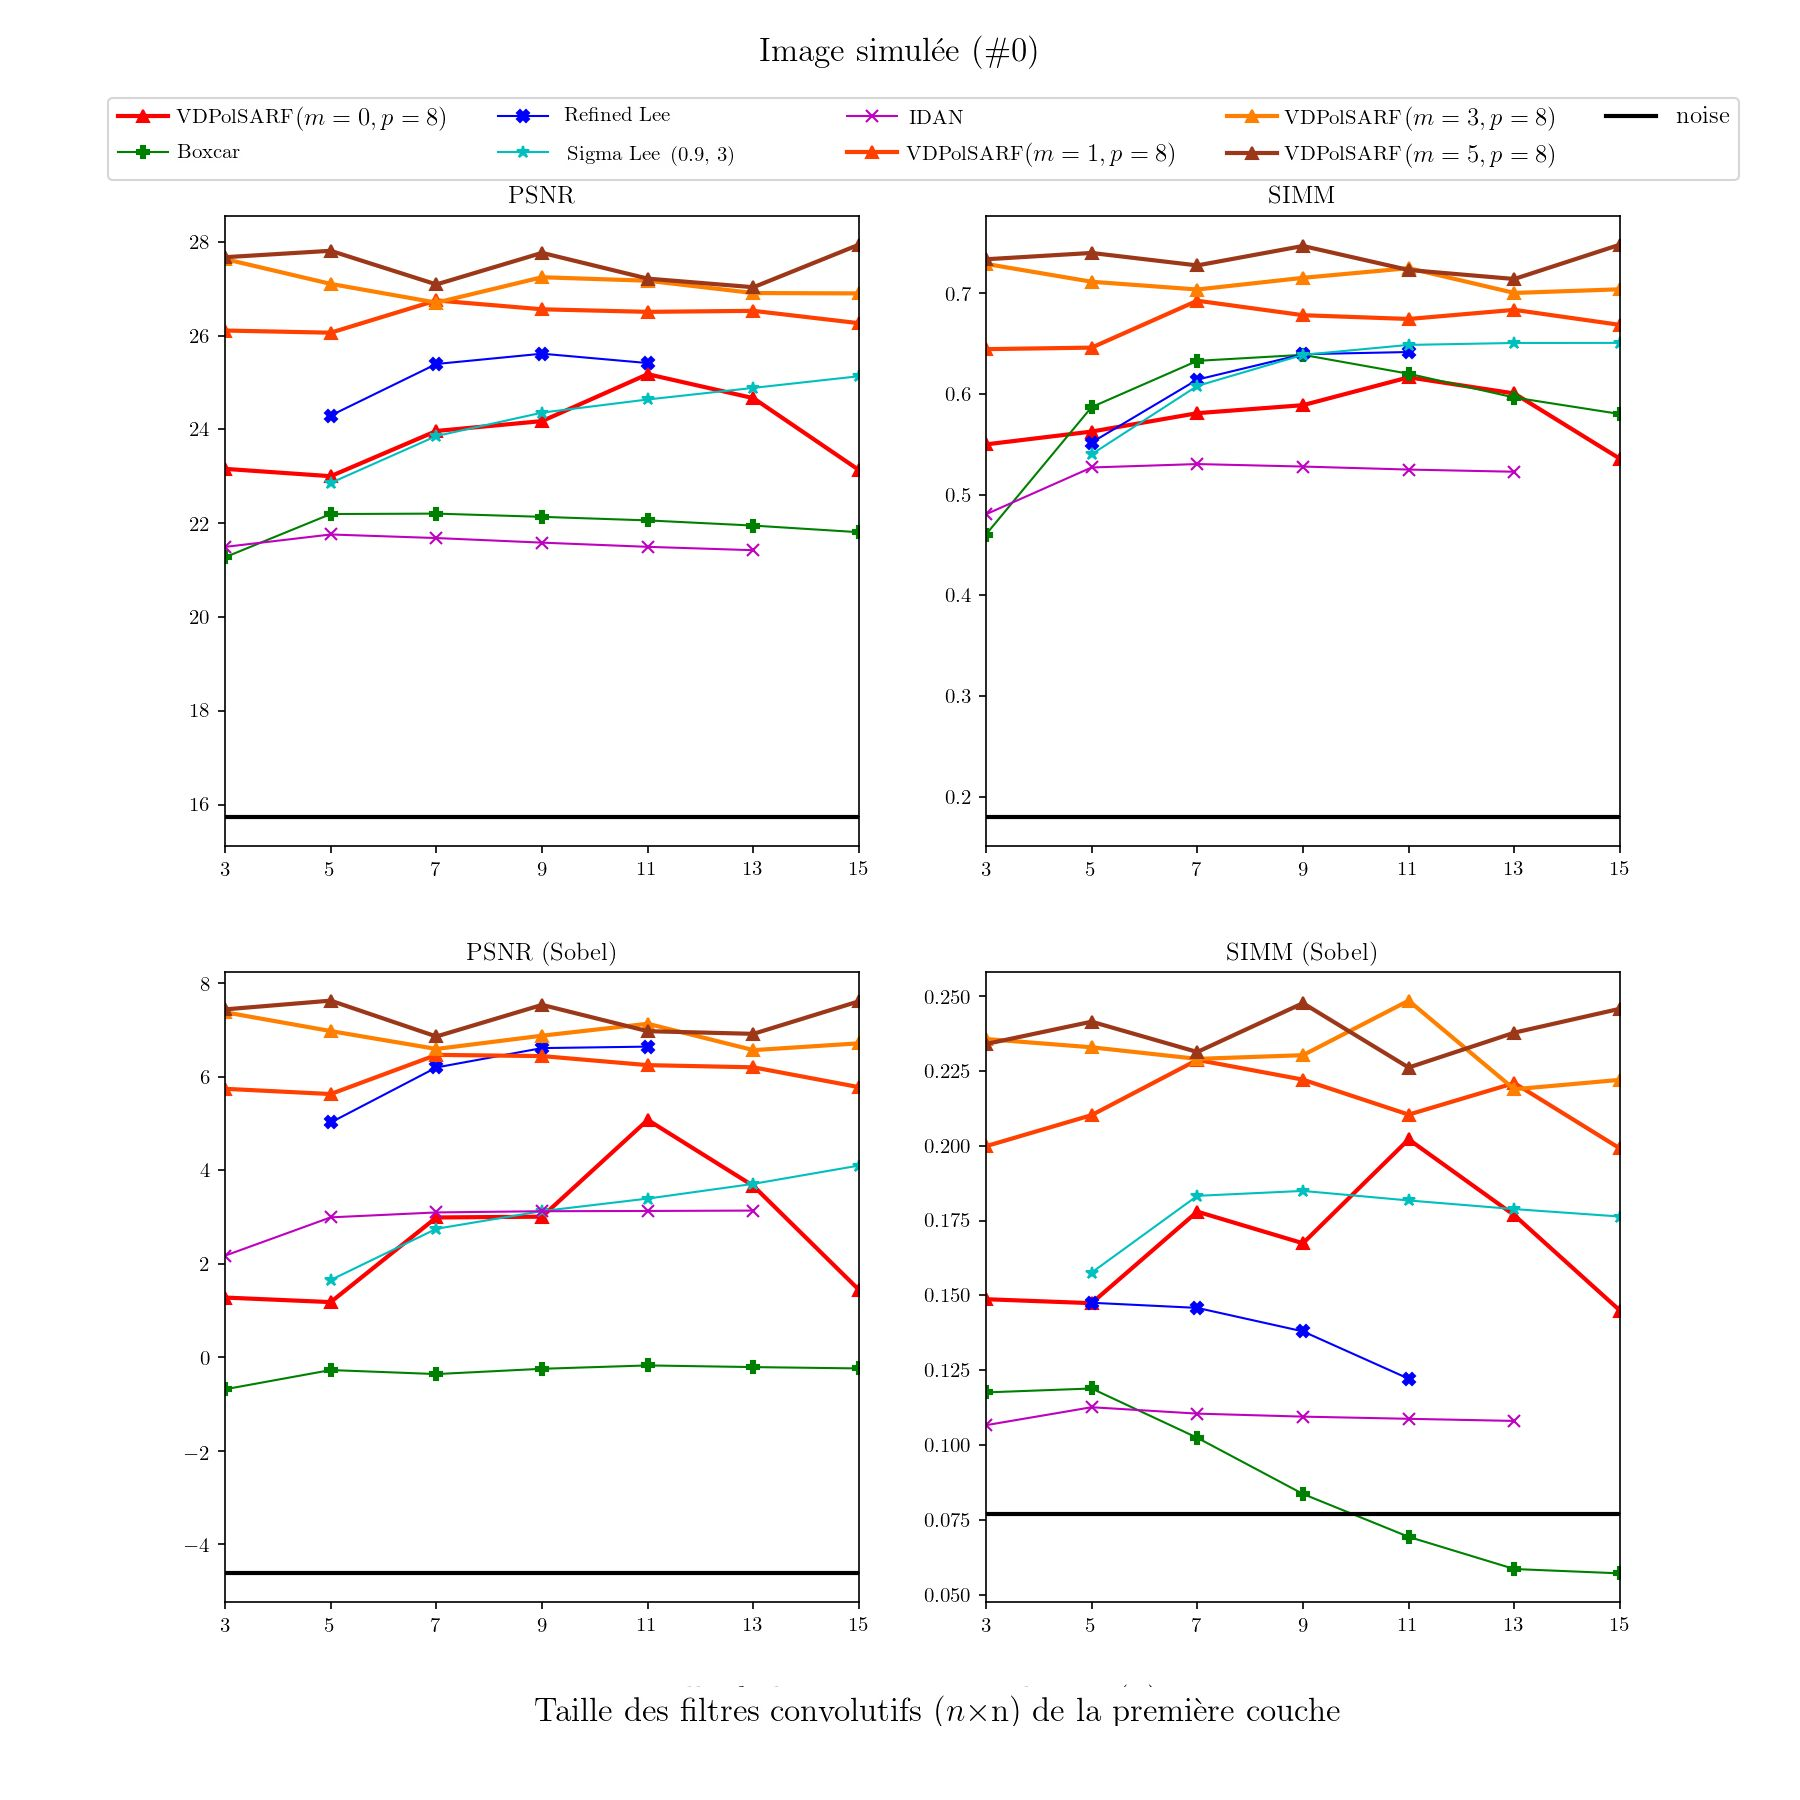
\includegraphics[width=1.0\textwidth]{figures/Chap4/results/analyse_multi_sigs/psnr/img_multipolsar_000_noised.jpg}
 \centering
  \caption{
  \footnotesize{  \textbf{Image simulée 0)}. Moyenne du \textbf{PSNR} et du \textbf{SSIM} sur l'image du \textbf{span} et sur l'image de Sobel du \textbf{span}.  Les résultats sont présentés en fonction de la taille $n$ de l'entrée des filtres.
  }
  }
  \label{fig:filter_psnr_0}
\end{figure}

Dans le cas du \textbf{PSNR} sur les images de Sobel, nous observons que les performances sont faibles avec des scores inférieurs à 8.  Les performances se séparent en trois groupes: le filtre \textbf{Boxcar}, les filtres "standards" avec le filtre \textbf{VDPolSARF} le plus court et les filtres appris plus profonds \textbf{VDPolSARF} ($m=1,3,5$).  Par contre pour l'image \#0 où le filtre \textbf{Refined LEE} rejoint les performances du filtre  \textbf{VDPolSARF} ($m=3$).

\begin{figure}[!htbp] 
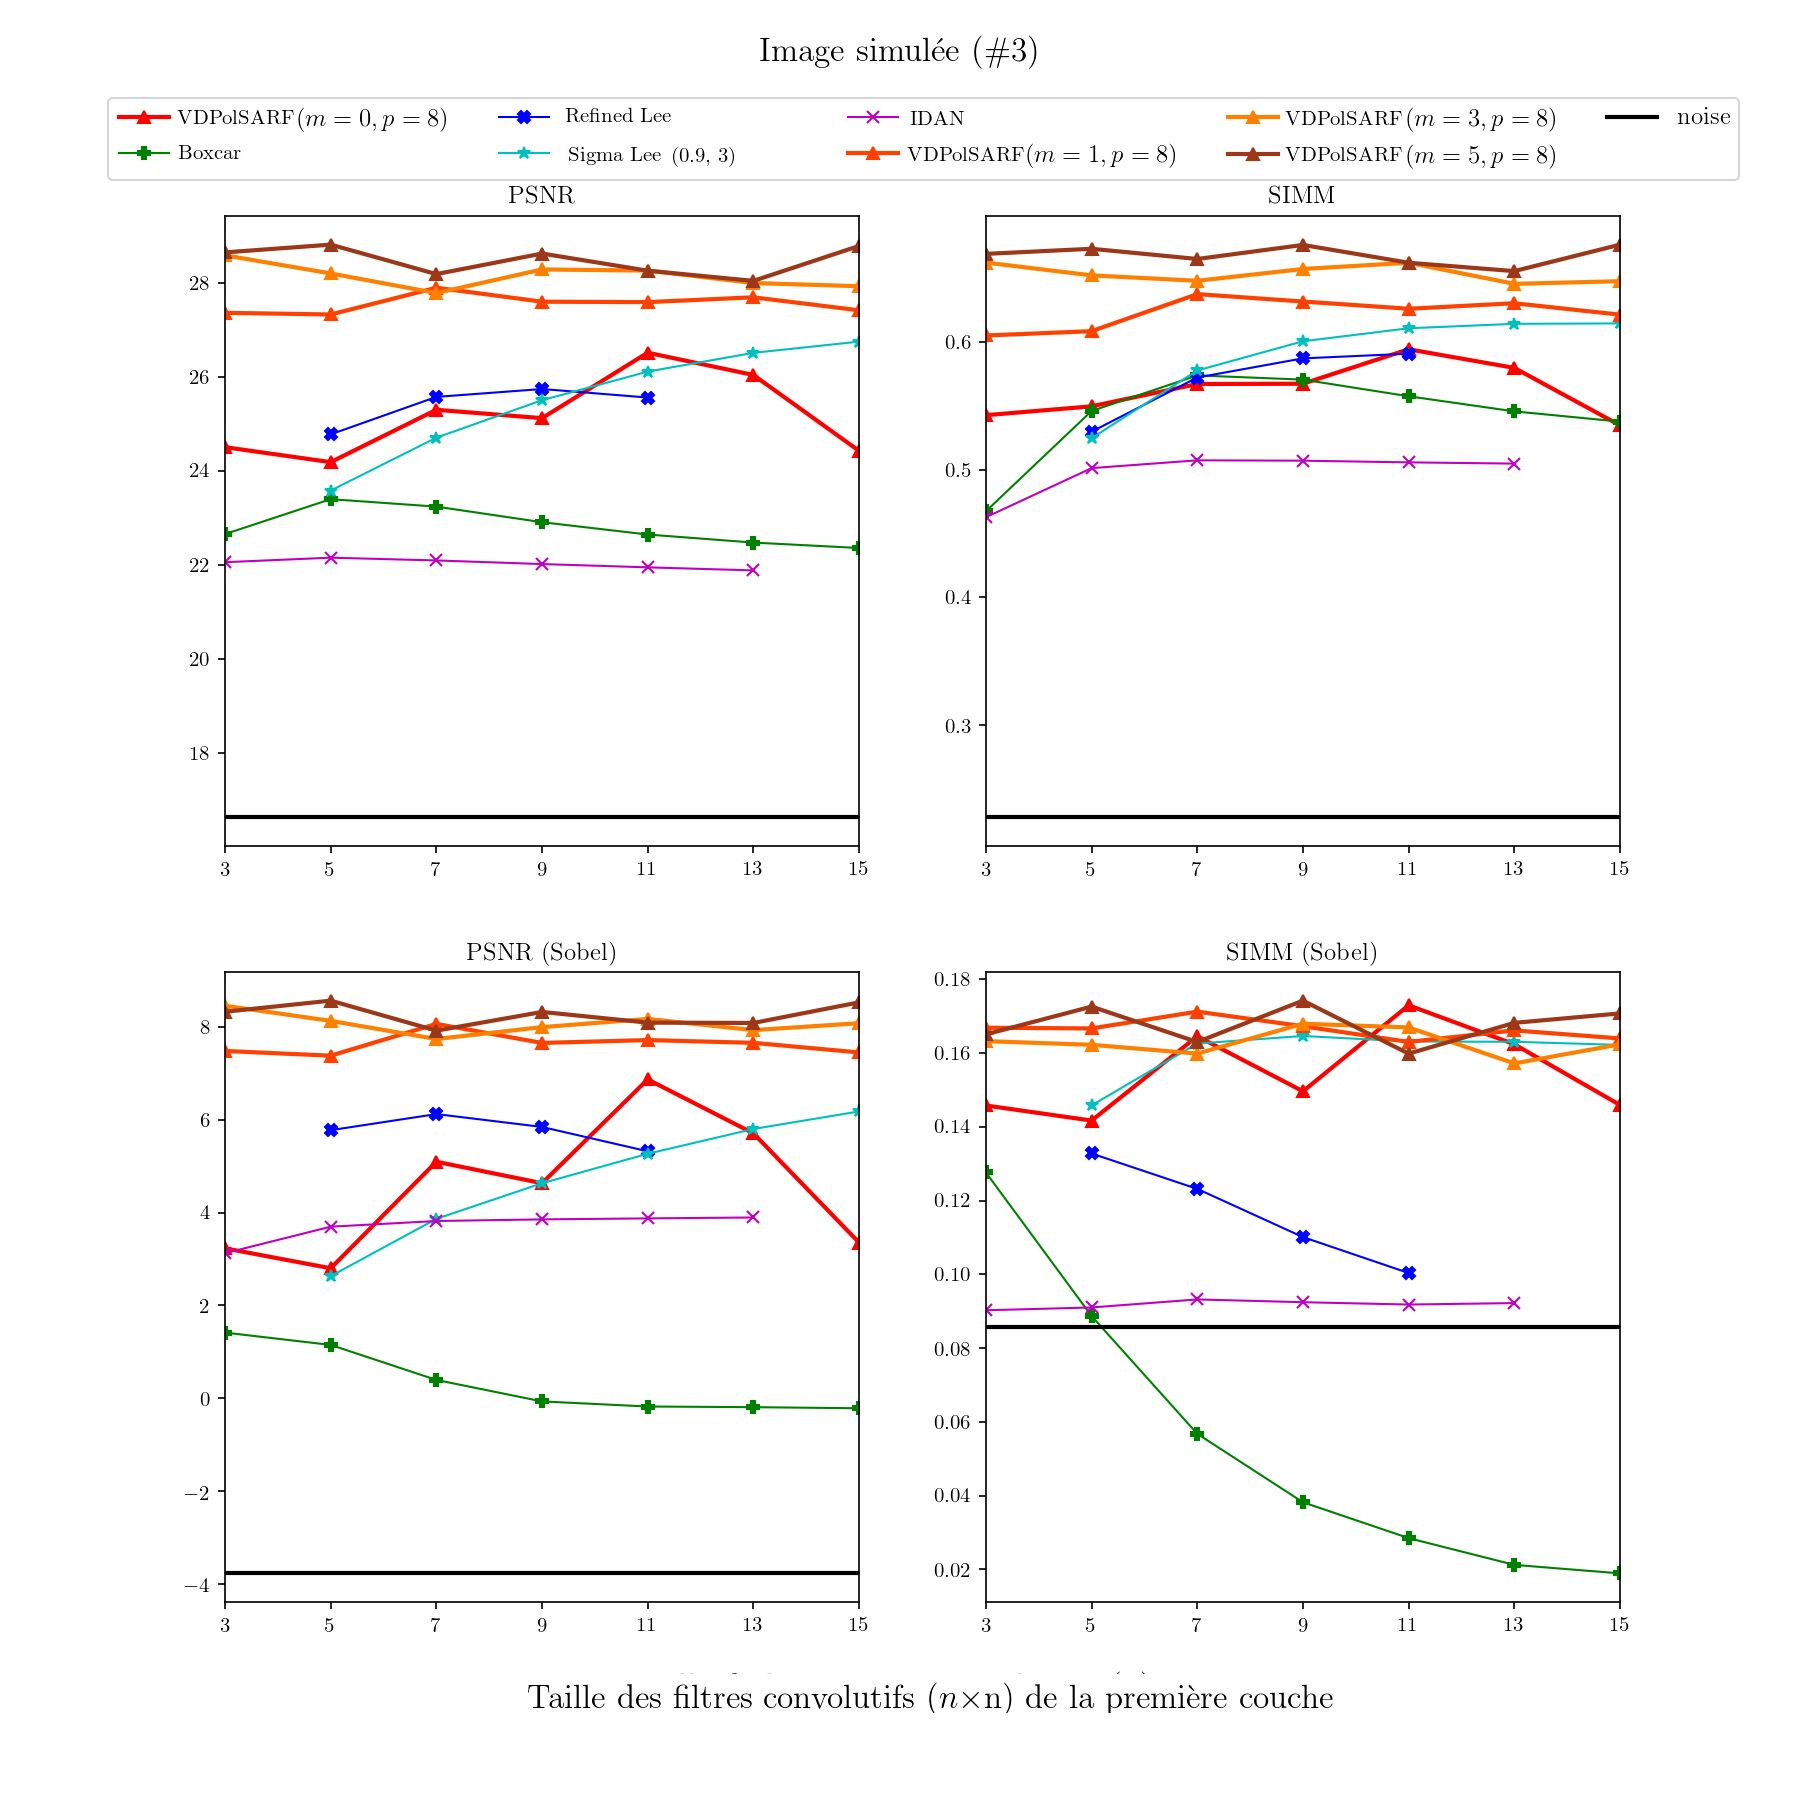
\includegraphics[width=1.0\textwidth]{figures/Chap4/results/analyse_multi_sigs/psnr/img_multipolsar_003_noised.jpg}
 \centering
  \caption{
  \footnotesize{  \textbf{Image simulée 3}. Moyenne du \textbf{PSNR} et du \textbf{SSIM} sur l'image du \textbf{span} et sur l'image de Sobel du \textbf{span}.  Les résultats sont présentés en fonction de la taille $n$ des filtres.
  }}
  \label{fig:filter_psnr_3}
\end{figure}

Dans le cas des résultats des \textbf{SSIM} sur les images filtrées et des \textbf{SSIM} sur les images filtrées de Sobel, nos observations sont semblables à celles émises pour les \textbf{PSNR}. De manière systématique les filtres appris les plus profonds \textbf{VDPolSARF} obtiennent les meilleurs performances si nous les comparons aux filtres "standards" et au filtre \textbf{Boxcar}.


\section{La qualité de la restitution des cibles ponctuelles}

Cette section présente quelques résultats montrant la capacité des algorithmes à préserver les cibles ponctuelles. Nous avons comparé la conservation de la superficie des cibles entre les différentes approches.  La Figure \ref{fig:filter_target_surface} schématise les trois mesures que nous avons réalisées. Si nous considérons la surface A comme la cible étiquette et forme B comme la cible restituée, nous pouvons calculer les mesures suivantes:

\begin{enumerate}
    \item La superficie préservée: superficie($A \cap B$) / superficie($A$)
    \item La superficie additionnée: superficie($B / (A \cap B$)) / superficie($A$)
    \item La superficie supprimée: superficie($A / (A \cap B$)) / superficie($A$)
\end{enumerate}

\begin{figure}[!htbp] 
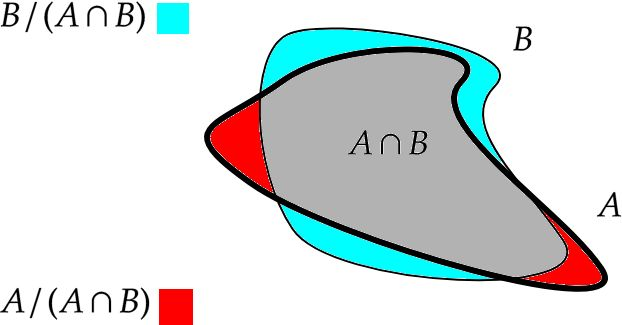
\includegraphics[width=0.5\textwidth]{figures/Chap4/results/targets.jpg}
 \centering
  \caption{
  \small{Schéma représentant les changements possibles de la géométrie de la cible.    }}
  \label{fig:filter_target_surface}
\end{figure}

Les Figures \ref{fig:filter_target_comparison_image_000_2} et \ref{fig:filter_target_comparison_image_003_2} montrent l'analyse sur nos deux images synthétiques.  Nous comparons les résultats obtenus avec le modèle \textbf{VDPolSARF} ($m=5, p=8)$ et le filtre \textbf{Boxcar} pour deux tailles de fenêtre $n=5, 13$. Les images ont été seuillées à 3 dB afin de ne conserver que les cibles ponctuelles. Nous observons les résultats prévisibles du \textbf{Boxcar} qui perd graduellement les cibles en fonction de la taille du filtre.  Dans le cas du filtre $13 \times 13$ les cibles sont complètement diluées. Dans le cas des filtres appris, les résultats varient entre 99.8 \% et  93.8 \% de préservation des cibles pour la taille de fenêtre de $5 \times 5$ et de 100 \% à 96.5 \% pour une taille de fenêtre de $13 \times 13$.

\targetresultsmultisigs{000}{0}
\targetresultsmultisigs{003}{3}

%%%%%%%%%%%%%%%%%%%%%%%%%%%%%%%%%%%%%%%%%%%%%%%%%%%%%%%%%%%%%%%%%%%%%%%%%%%%%%%%%%%%%%%%%%%%%%%%%%%%%%%%%%%%%%%

\section{L'effet de la complexité de l'apprentissage sur l'estimation des paramètres polarimétriques}
Cette dernière section sur les données synthétiques met en relief l'effet du type d'apprentissage sur les résultats des estimées des paramètres polarimétriques sur des surfaces homogènes. Nous rappelons que les apprentissages ont été faits sous les mêmes conditions (Sec. \ref{sec:experimental_protocol}). La seule variable qui a changé est l'ensemble de données utilisé pour les apprentissages.  Afin d'observer l'influence sur chacun des paramètres estimés, nous avons refait les analyses sur les régions homogènes mais en utilisant les modèles entraînés sur les données hétérogènes et les modèles entraînés sur les données hétérogènes avec inclusion de cibles ponctuelles.  Nous ne présentons que les résultats sur le diffuseur \textit{double bond} car les résultats sont similaires pour les autres types de diffuseurs.  Les Figures \ref{figB:Double_Reflection_homogeneous}, \ref{figB:Double_Reflection_random_texture}, \ref{figB:Double_Reflection_random_texture_with_pts} présentent le biais estimé sur les termes de la matrice de cohérence.   Les Figures \ref{figB:enl_Double_Reflection_homogeneous}, \ref{figB:enl_Double_Reflection_random_texture}, \ref{figB:enl_Double_Reflection_random_texture_with_pts} présentent les valeurs du \textbf{NEV} sur les termes diagonaux de la matrice de cohérence et les Figures \ref{figB:haalpha_Double_Reflection_homogeneous}, \ref{figB:haalpha_Double_Reflection_random_texture}, \ref{figB:haalpha_Double_Reflection_random_texture_with_pts} présentent les biais calculés sur les paramètres de la décomposition de \haalpha.

Nous remarquons la tendance générale de la perte de performance en fonction de la complexité des données d'apprentissage. Le passage entre l'apprentissage à partir des données homogènes et les données hétérogènes pour l'estimation des termes de la matrice de cohérence et des paramètres de la décomposition de \halpha montrent une légère perte de performance de l'ordre de 2 \%.  Dans le cas du calcul du \textbf{NEV} on observe une perte de plus de 35 \% pour le modèle ($m=5, p=8$, $n=3$) et de plus de 50 \% pour le modèle ($m=5, p=8$, $n=15$).  Cependant les résultats demeurent supérieurs aux autres filtres "standards" et au filtre \textbf{Boxcar} pour les modèles \textbf{VDPolSARF} ($m=3,5$, $p=8$ et $n < 9$).

L'introduction de cibles ponctuelles affecte de façon notoire les résultats des modèles courts ($m=0, m=1,3$) et nuisent plus aux modèles avec une large fenêtre d'entrée $n > 9$.  On remarque que les modèles profonds ($m=5$, $p=8$, $n<9$) réussissent malgré tout à maintenir de bons estimés pour les termes de la matrice de cohérence et les paramètres \haalphaB. Les valeurs du \textbf{NEV} demeurent supérieures pour des tailles de fenêtre inférieures ou égales à 9 si nous les comparons aux filtres "standards". 

La Figure \ref{figB:training_comparison_Double_Reflection} montre un exemple visuel qui met en relief l'influence des données d'apprentissage sur la capacité des modèles à filtrer les régions homogènes.

\matcohfigavgallB{all}{8}{Double_Reflection_homogeneous}{homogeneous}{(apprentissage sur les données homogènes).}{Double_Reflection}{Diffuseurs}{double bond}{homogeneous}

\matcohfigavgallB{all}{8}{Double_Reflection_random_texture}{homogeneous}{(apprentissage sur les données hétérogènes).}{Double_Reflection}{Diffuseurs}{double bond}{random_texture}

\matcohfigavgallB{all}{8}{Double_Reflection_random_texture_with_pts}{homogeneous}{(apprentissage sur les données hétérogènes avec inclusion de cibles ponctuelles)}{Double_Reflection}{Diffuseurs}{double bond}{random_texture_with_pts}

\enlfiguresB{Double_Reflection}{Diffuseurs}{double bond}{homogeneous}{(apprentissage sur les données homogènes)}

\enlfiguresB{Double_Reflection}{Diffuseurs}{double bond}{random_texture}{(apprentissage sur les données hétérogènes)}

\enlfiguresB{Double_Reflection}{Diffuseurs}{double bond}{random_texture_with_pts}{(apprentissage sur les données hétérogènes avec inclusion de cibles ponctuelles)}

\haalphafigavgallB{all}{8}{haalpha_Double_Reflection_homogeneous}{homogeneous_haalpha}{(apprentissage sur les données homogènes)}{Double_Reflection}{Diffuseurs}{double bond}{homogeneous}

\haalphafigavgallB{all}{8}{haalpha_Double_Reflection_random_texture}{homogeneous_haalpha}{(apprentissage sur les données hétérogènes)}{Double_Reflection}{Diffuseurs}{double bond}{random_texture}


\haalphafigavgallB{all}{8}{haalpha_Double_Reflection_random_texture_with_pts}{homogeneous_haalpha}{(apprentissage sur les données hétérogènes avec inclusion de cibles ponctuelles)}{Double_Reflection}{Diffuseurs}{double bond}{random_texture_with_pts}

\vdtrainingcompare{signature_Double_Reflection}{Diffuseurs}{double bond}{2}{Double_Reflection}

%%%%%%%%%%%%%%%%%%%%%%%%%%%%%%%%%%%%%%%%%%%%%%%%%%%%%%%%%%%%%%%%%%%%%%%%%%%%%%%%%%%%%%%%%%%%%%%%%%%%%%%%%%%%%%%

\section{Évaluation qualitative sur les images polarimétriques réelles} \label{sec:Evaluation_qualitative_sur_les_images_polarimetriques_reelles}

Cette section présente l'application des modèles entraînés sur nos images polarimétriques test.  Ces images ont été décrites à la section \ref{section:données_réelles}.  Les Figures \ref{fig:plate_1_RADARSAT2_1_(1)_n0=9_n=9} et \ref{fig:plate_2_RADARSAT2_1_(2)_n0=9_n=9}, \ref{fig:plate_1_ALOS2_1_(1)_n0=9_n=9} et \ref{fig:plate_2_ALOS2_1_(2)_n0=9_n=9}, \ref{fig:plate_1_GAF3_1_(1)_n0=9_n=9} et \ref{fig:plate_2_GAF3_1_(2)_n0=9_n=9} illustrent les résultats sur l'image en QuadPol RADARSAT2, ALOS2 et GAF3. Nous y comparons le modèle \textbf{VDPolSARF} ($m=5, p=8, n=9$) entraîné sur les données hétérogènes et le même modèle \textbf{VDPolSARF} ($m=5, p=8, n=9$) entraîné sur les données hétérogènes avec inclusion de cibles ponctuelles par rapport aux différents filtres polarimétriques standards. A cette échelle les résultats semblent assez bien filtrés par nos deux modèles \textbf{VDPolSARF} (Figs. \ref{fig:plate_1_RADARSAT2_1_(1)_n0=9_n=9}, \ref{fig:plate_1_ALOS2_1_(1)_n0=9_n=9} et \ref{fig:plate_1_GAF3_1_(1)_n0=9_n=9} (b) et (c) ), ils sont comparables aux résultats du filtre \textbf{Sigma Lee} (Fig. \ref{fig:plate_1_RADARSAT2_1_(1)_n0=9_n=9} (d)). Nous donnons aussi les résultats du  modèle \textbf{VDPolSARF} ($m=5, p=8, n=9$) entraîné sur les données homogènes   (Figs. \ref{fig:plate_2_RADARSAT2_1_(2)_n0=9_n=9}, \ref{fig:plate_2_ALOS2_1_(2)_n0=9_n=9} et \ref{fig:plate_2_GAF3_1_(2)_n0=9_n=9} (d)) à titre de comparaison avec le filtre Boxcar 9x9 (Figs. \ref{fig:plate_2_RADARSAT2_1_(2)_n0=9_n=9}, \ref{fig:plate_2_ALOS2_1_(2)_n0=9_n=9} et \ref{fig:plate_2_GAF3_1_(2)_n0=9_n=9} (c)). Nous pouvons dès lors remarquer que ce modèle filtre beaucoup plus les zones homogènes que tous les autres modèles entraînés ainsi que les autres filtres standards et le filtre \textbf{Boxcar}.  Par contre il crée de nombreux artéfacts autour des cibles ponctuelles. Ce qui est normal, puisque l'apprentissage a été effectué sur des images complètement homogènes.

\filterscomparefig{1}{RADARSAT2}{1}{(1)}
\filterscomparefig{2}{RADARSAT2}{1}{(2)}

\filterscomparefig{1}{ALOS2}{1}{(1)}
\filterscomparefig{2}{ALOS2}{1}{(2)}

\filterscomparefig{1}{GAF3}{1}{(1)}
\filterscomparefig{2}{GAF3}{1}{(2)}

Maintenant, lorsque nous analysons plus attentivement les résultats à plus grande échelle (Figs. \ref{fig:plate_1_RADARSAT2_3_(1)_n0=9_n=9},  \ref{fig:plate_1_ALOS2_3_(1)_n0=9_n=9} et \ref{fig:plate_1_GAF3_3_(1)_n0=9_n=9}), nous pouvons remarquer que chacun de nos deux modèles produit des résultats quelques peu différents.  Premièrement le modèle entraîné sur les données hétérogènes semble meilleur pour filtrer les zones homogènes, par contre les cibles ponctuelles sont dégradées quelque peu par des artefacts sur le pourtour des cibles.  On le remarque particulièrement sur l'image ALOS2 (Fig. \ref{fig:plate_1_ALOS2_3_(1)_n0=9_n=9} (b)).  Dans le cas de notre second modèle, il préserve assez bien les cibles mais il semble ne pas suffisamment filtrer les régions homogènes.  On remarque une forme de pixelisation qui est particulièrement visible sur l'image de RADARSAT2 (\ref{fig:plate_1_RADARSAT2_3_(1)_n0=9_n=9} (c)) et GAF3 (\ref{fig:plate_1_GAF3_3_(1)_n0=9_n=9} (c)).  Sur le plan de la préservation des détails, nos modèles entraînés semblent donner des résultats aussi bons que le filtre \textbf{Sigma Lee}. Il nous apparaît que le modèle \textbf{VDPolSARF} ($m=5, p=8, n=9$) entraîné sur les données hétérogènes donne de meilleurs résultats sur les images ALOS2 pour la préservation des arêtes que les autres filtres.

%\filterscomparefigh{1}{RADARSAT2}{2}{(1)}
%\filterscomparefigh{2}{RADARSAT2}{2}{(2)}

\filterscomparefigh{1}{RADARSAT2}{3}{(1)}
%\filterscomparefigh{2}{RADARSAT2}{3}{(2)}

%\imagesubregion{ALOS2}{1}
%\imagesubregionfiltered{ALOS2}{1}

%\filterscomparefigh{1}{ALOS2}{2}{(1)}
%\filterscomparefigh{2}{ALOS2}{2}{(2)}

\filterscomparefigh{1}{ALOS2}{3}{(1)}
%\filterscomparefigh{2}{ALOS2}{3}{(2)}

%\imagesubregion{GAF3}{1}
%\imagesubregionfiltered{GAF3}{1}

%\filterscomparefigh{1}{GAF3}{2}{(1)}
%\filterscomparefigh{2}{GAF3}{2}{(2)}

\filterscomparefigh{1}{GAF3}{3}{(1)}
%\filterscomparefigh{2}{GAF3}{3}{(2)}

\section{Évaluation du nombre équivalent de vues sur les images polarimétriques réelles}

Les tableaux suivants (Tab.  \ref{tab:radarsat2_results_table}, \ref{tab:alos2_results_table} et \ref{tab:gaf3_results_table}) présentent le nombre équivalent de vues calculé pour chacune de nos expérimentations.  Sur chaque image polarimétrique nous avons sélectionné la même région homogène et exécuté le calcul sur les éléments en puissance des matrices de cohérence.  Pour chacun des capteurs, nous obtenons des résultats supérieurs avec le modèle \textbf{VDPolSARF} ($m=5, p=8, n=9$) entraîné sur les données hétérogènes par rapport aux filtres standards (\textbf{Sigma Lee}, \textbf{Refined Lee }et \textbf{IDAN}). Il n'est dépassé que par le \textbf{Boxcar}, sauf dans le cas des données ALOS2.  Les résultats pour le modèle \textbf{VDPolSARF} ($m=5, p=8, n=9$) entraîné sur les données hétérogènes avec inclusion de cible corrobore notre problème de sous-filtrage identifié à la section précédente (sec. \ref{sec:Evaluation_qualitative_sur_les_images_polarimetriques_reelles}).  Les résultats sont nettement inférieurs à nos attentes.  Dans le cas du  modèle \textbf{VDPolSARF} ($m=5, p=8, n=9$) entraîné sur le données homogènes, il démontrent nettement son efficacité à filtrer les zones homogènes. Les \textbf{NEV} obtenus sont nettement supérieurs au \textbf{Boxcar}.  Ce qui confirme nos résultats précédents sur la qualité du filtrage.

\vspace{5pt}

\begin{table}[!htbp]
\tiny
\centering
\begin{tabular}{c|c|c|c|c|c|c|c|c|c|c|c|c|}
\cline{2-13}
                                        & \multicolumn{3}{c|}{\textbf{POLSAR}}                                                             & \multicolumn{3}{c|}{\textbf{\begin{tabular}[c]{@{}c@{}}\textbf{VDPolSARF} \\ (m=5, p=8, n=9)\\ hétérogène\end{tabular}}} & \multicolumn{3}{c|}{\textbf{\begin{tabular}[c]{@{}c@{}}\textbf{VDPolSARF} \\ (m=5, p=8, n=9)\\ hétérogène + cibles\end{tabular}}} & \multicolumn{3}{c|}{\textbf{\begin{tabular}[c]{@{}c@{}}\textbf{Sigma Lee}\\ $9 \times 9$\end{tabular}}}         \\ \hline
\multicolumn{1}{|c|}{\textbf{}}         & \textbf{$\mu$}                & \textbf{$\sigma$}                & \textbf{NEV}                  & \textbf{$\mu$}                    & \textbf{$\sigma$}                   & \textbf{NEV}                     & \textbf{$\mu$}                      & \textbf{$\sigma$}                      & \textbf{NEV}                        & \textbf{$\mu$}                   & \textbf{$\sigma$}                   & \textbf{NEV}                    \\ \hline
\multicolumn{1}{|c|}{\textbf{$T_{11}$}} & 2.24e-01                      & 2.50e-01                         & \textbf{0.80}                 & 2.19e-01                          & 5.63e-02                            & \textbf{15.19}                   & 2.22e-01                            & 1.48e-01                               & \textbf{2.25}                       & 2.08e-01                         & 7.70e-02                            & \textbf{7.31}                   \\ \hline
\multicolumn{1}{|c|}{\textbf{$T_{22}$}} & 8.38e-03                      & 8.73e-03                         & \textbf{0.92}                 & 8.27e-03                          & 1.76e-03                            & \textbf{22.06}                   & 8.34e-03                            & 4.12e-03                               & \textbf{4.09}                       & 7.90e-03                         & 2.40e-03                            & \textbf{10.80}                  \\ \hline
\multicolumn{1}{|c|}{\textbf{$T_{33}$}} & 2.11e-03                      & 2.24e-03                         & \textbf{0.88}                 & 2.06e-03                          & 4.85e-04                            & \textbf{18.08}                   & 2.09e-03                            & 1.12e-03                               & \textbf{3.50}                       & 1.96e-03                         & 5.86e-04                            & \textbf{11.13}                  \\ \hline
\textbf{}                               & \multicolumn{3}{c|}{\textbf{\begin{tabular}[c]{@{}c@{}}\textbf{Refined Lee}\\ $9 \times 9$\end{tabular}}} & \multicolumn{3}{c|}{\textbf{\begin{tabular}[c]{@{}c@{}}\textbf{IDAN}\\ pixels=81\end{tabular}}}                     & \multicolumn{3}{c|}{\textbf{\begin{tabular}[c]{@{}c@{}}\textbf{Boxcar}\\ $9 \times 9$\end{tabular}}}                        & \multicolumn{3}{c|}{\textbf{\begin{tabular}[c]{@{}c@{}}\textbf{VDPolSARF}  \\ (m=5, p=8, n=9)\\ homogène\end{tabular}}} \\ \hline
\multicolumn{1}{|c|}{\textbf{$T_{11}$}} & 1.84e-01                      & 5.64e-02                         & \textbf{10.69}                & 1.54e-01                          & 5.39e-02                            & 8.19                             & 2.23e-01                            & 4.55e-02                               & \textbf{24.13}                      & 2.22e-01                         & 2.99e-02                            & \textbf{55.07}                  \\ \hline
\multicolumn{1}{|c|}{\textbf{$T_{22}$}} & 7.95e-03                      & 1.99e-03                         & \textbf{15.98}                & 6.14e-03                          & 2.02e-03                            & 9.27                             & 8.40e-03                            & 1.46e-03                               & \textbf{33.17}                      & 8.40e-03                         & 8.90e-04                            & \textbf{89.08}                  \\ \hline
\multicolumn{1}{|c|}{\textbf{$T_{33}$}} & 2.05e-03                      & 5.35e-04                         & \textbf{14.73}                & 1.57e-03                          & 5.31e-04                            & 8.71                             & 2.09e-03                            & 3.97e-04                               & \textbf{27.75}                      & 2.09e-03                         & 2.50e-04                            & \textbf{69.45}                  \\ \hline
\end{tabular}
\caption{\small{Mesure du nombre équivalent de vues sur une zone de type surfacique sur les termes en puissance de l'image RADARSAT2.  La moyenne, l'écart-type et le \textbf{NEV} est calculé pour chaque filtre.}}
\label{tab:radarsat2_results_table}
\end{table}


\begin{table}[!htbp]
\tiny
\centering
\begin{tabular}{c|c|c|c|c|c|c|c|c|c|c|c|c|}
\cline{2-13}
                                        & \multicolumn{3}{c|}{\textbf{POLSAR}}                                                             & \multicolumn{3}{c|}{\textbf{\begin{tabular}[c]{@{}c@{}}\textbf{VDPolSARF} \\ (m=5, p=8, n=9)\\ hétérogène\end{tabular}}} & \multicolumn{3}{c|}{\textbf{\begin{tabular}[c]{@{}c@{}}\textbf{VDPolSARF} \\ (m=5, p=8, n=9)\\ hétérogène + cibles\end{tabular}}} & \multicolumn{3}{c|}{\textbf{\begin{tabular}[c]{@{}c@{}}\textbf{Sigma Lee}\\ $9 \times 9$\end{tabular}}}         \\ \hline
\multicolumn{1}{|c|}{\textbf{}}         & \textbf{$\mu$}                & \textbf{$\sigma$}                & \textbf{NEV}                  & \textbf{$\mu$}                    & \textbf{$\sigma$}                   & \textbf{NEV}                     & \textbf{$\mu$}                      & \textbf{$\sigma$}                      & \textbf{NEV}                        & \textbf{$\mu$}                   & \textbf{$\sigma$}                   & \textbf{NEV}                    \\ \hline
\multicolumn{1}{|c|}{\textbf{$T_{11}$}} & 7.33e-02                      & 7.74e-02                         & \textbf{0.90}                 & 7.26e-02                          & 1.79e-02                            & \textbf{16.42}                   & 7.30e-02                            & 2.47e-02                               & \textbf{8.76}                       & 6.98e-02                         & 2.17e-02                            & \textbf{10.38}                  \\ \hline
\multicolumn{1}{|c|}{\textbf{$T_{22}$}} & 1.60e-02                      & 1.61e-02                         & \textbf{0.99}                 & 1.59e-02                          & 2.43e-03                            & \textbf{43.09}                   & 1.60e-02                            & 3.22e-03                               & \textbf{24.71}                      & 1.54e-02                         & 3.65e-03                            & \textbf{17.93}                  \\ \hline
\multicolumn{1}{|c|}{\textbf{$T_{33}$}} & 3.82e-03                      & 3.84e-03                         & \textbf{0.99}                 & 3.80e-03                          & 5.92e-04                            & \textbf{41.24}                   & 3.81e-03                            & 6.44e-04                               & \textbf{35.03}                      & 3.71e-03                         & 8.93e-04                            & \textbf{17.20}                  \\ \hline
\textbf{}                               & \multicolumn{3}{c|}{\textbf{\begin{tabular}[c]{@{}c@{}}\textbf{Refined Lee}\\ $9 \times 9$\end{tabular}}} & \multicolumn{3}{c|}{\textbf{\begin{tabular}[c]{@{}c@{}}\textbf{IDAN}\\ pixels=81\end{tabular}}}                     & \multicolumn{3}{c|}{\textbf{\begin{tabular}[c]{@{}c@{}}\textbf{Boxcar}\\ $9 \times 9$\end{tabular}}}                        & \multicolumn{3}{c|}{\textbf{\begin{tabular}[c]{@{}c@{}}\textbf{VDPolSARF}  \\ (m=5, p=8, n=9)\\ homogène\end{tabular}}} \\ \hline
\multicolumn{1}{|c|}{\textbf{$T_{11}$}} & 6.20e-02                      & 1.69e-02                         & \textbf{13.39}                & 5.59e-02                          & 1.92e-02                            & 8.45                             & 7.33e-02                            & 1.77e-02                               & \textbf{17.14}                      & 7.33e-02                         & 1.46e-02                            & \textbf{25.19}                  \\ \hline
\multicolumn{1}{|c|}{\textbf{$T_{22}$}} & 1.53e-02                      & 3.14e-03                         & \textbf{23.83}                & 1.25e-02                          & 3.57e-03                            & 12.25                            & 1.60e-02                            & 2.63e-03                               & \textbf{37.27}                      & 1.60e-02                         & 1.77e-03                            & \textbf{81.50}                  \\ \hline
\multicolumn{1}{|c|}{\textbf{$T_{33}$}} & 3.76e-03                      & 7.76e-04                         & \textbf{23.53}                & 3.05e-03                          & 8.85e-04                            & 11.84                            & 3.82e-03                            & 6.50e-04                               & \textbf{34.44}                      & 3.82e-03                         & 4.77e-04                            & \textbf{64.08}                  \\ \hline
\end{tabular}
\caption{\small{Mesure du nombre équivalent de vues équivalent sur une zone de type surfacique sur les termes en puissance de l'image ALOS2.  La moyenne, l'écart-type et le \textbf{NEV} est calculé pour chaque filtre.}}
\label{tab:alos2_results_table}
\end{table}


\begin{table}[!htbp]
\tiny
\centering
\begin{tabular}{c|c|c|c|c|c|c|c|c|c|c|c|c|}
\cline{2-13}
                                        & \multicolumn{3}{c|}{\textbf{POLSAR}}                                                             & \multicolumn{3}{c|}{\textbf{\begin{tabular}[c]{@{}c@{}}\textbf{VDPolSARF} \\ (m=5, p=8, n=9)\\ hétérogène\end{tabular}}} & \multicolumn{3}{c|}{\textbf{\begin{tabular}[c]{@{}c@{}}\textbf{VDPolSARF} \\ (m=5, p=8, n=9)\\ hétérogène + cibles\end{tabular}}} & \multicolumn{3}{c|}{\textbf{\begin{tabular}[c]{@{}c@{}}\textbf{Sigma Lee}\\ $9 \times 9$\end{tabular}}}         \\ \hline
\multicolumn{1}{|c|}{\textbf{}}         & \textbf{$\mu$}                & \textbf{$\sigma$}                & \textbf{NEV}                  & \textbf{$\mu$}                    & \textbf{$\sigma$}                   & \textbf{NEV}                     & \textbf{$\mu$}                      & \textbf{$\sigma$}                      & \textbf{NEV}                        & \textbf{$\mu$}                   & \textbf{$\sigma$}                   & \textbf{NEV}                    \\ \hline
\multicolumn{1}{|c|}{\textbf{$T_{11}$}} & 6.18e-01                      & 7.16e-01                         & \textbf{0.74}                 & 6.05e-01                          & 1.97e-01                            & \textbf{9.47}                    & 6.14e-01                            & 4.02e-01                               & \textbf{2.33}                       & 5.74e-01                         & 2.48e-01                            & \textbf{5.36}                   \\ \hline
\multicolumn{1}{|c|}{\textbf{$T_{22}$}} & 1.07e-02                      & 1.13e-02                         & \textbf{0.90}                 & 1.06e-02                          & 2.53e-03                            & \textbf{17.55}                   & 1.07e-02                            & 5.30e-03                               & \textbf{4.05}                       & 1.02e-02                         & 3.42e-03                            & \textbf{8.82}                   \\ \hline
\multicolumn{1}{|c|}{\textbf{$T_{33}$}} & 1.25e-03                      & 1.30e-03                         & \textbf{0.92}                 & 1.23e-03                          & 3.32e-04                            & \textbf{13.72}                   & 1.24e-03                            & 7.00e-04                               & \textbf{3.15}                       & 1.18e-03                         & 3.94e-04                            & \textbf{8.98}                   \\ \hline
\textbf{}                               & \multicolumn{3}{c|}{\textbf{\begin{tabular}[c]{@{}c@{}}\textbf{Refined Lee}\\ $9 \times 9$\end{tabular}}} & \multicolumn{3}{c|}{\textbf{\begin{tabular}[c]{@{}c@{}}\textbf{IDAN}\\ pixels=89\end{tabular}}}                     & \multicolumn{3}{c|}{\textbf{\begin{tabular}[c]{@{}c@{}}\textbf{Boxcar}\\ $9 \times 9$\end{tabular}}}                        & \multicolumn{3}{c|}{\textbf{\begin{tabular}[c]{@{}c@{}}\textbf{VDPolSARF}  \\ (m=5, p=8, n=9)\\ homogène\end{tabular}}} \\ \hline
\multicolumn{1}{|c|}{\textbf{$T_{11}$}} & 5.03e-01                      & 1.79e-01                         & \textbf{7.94}                 & 4.09e-01                          & 1.70e-01                            & 5.80                             & 6.19e-01                            & 1.58e-01                               & \textbf{15.35}                      & 6.18e-01                         & 1.11e-01                            & \textbf{30.85}                  \\ \hline
\multicolumn{1}{|c|}{\textbf{$T_{22}$}} & 9.86e-03                      & 2.70e-03                         & \textbf{13.33}                & 7.69e-03                          & 2.59e-03                            & 8.78                             & 1.08e-02                            & 2.29e-03                               & \textbf{22.05}                      & 1.08e-02                         & 1.57e-03                            & \textbf{46.71}                  \\ \hline
\multicolumn{1}{|c|}{\textbf{$T_{33}$}} & 1.23e-03                      & 3.45e-04                         & \textbf{12.64}                & 9.54e-04                          & 3.34e-04                            & 8.15                             & 1.25e-03                            & 2.90e-04                               & \textbf{18.70}                      & 1.25e-03                         & 2.13e-04                            & \textbf{34.68}                  \\ \hline
\end{tabular}
\caption{\small{Mesure du nombre de vues équivalent sur une zone de type surfacique sur les termes en puissance de l'image GAF3.  La moyenne, l'écart-type et le \textbf{NEV} est calculé pour chaque filtre.}}
\label{tab:gaf3_results_table}
\end{table}

%%\section{Évaluation de la décomposition H-A-Alpha sur les images polarimétriques réelles}

\filterscomparefighaalpha{1}{RADARSAT2}{1}{(1)}
\filterscomparefighhaalpha{1}{RADARSAT2}{2}{(2)}
\filterscomparefighhaalpha{1}{RADARSAT2}{3}{(4)}
\filterscomparefighhaalpha{1}{RADARSAT2}{4}{(4)}

\filterscomparefighaalpha{1}{ALOS2}{1}{(1)}
\filterscomparefighhaalpha{1}{ALOS2}{2}{(2)}
\filterscomparefighhaalpha{1}{ALOS2}{3}{(4)}
\filterscomparefighhaalpha{1}{ALOS2}{4}{(4)}

\filterscomparefighaalpha{1}{GAF3}{1}{(1)}
\filterscomparefighhaalpha{1}{GAF3}{2}{(2)}
\filterscomparefighhaalpha{1}{GAF3}{3}{(4)}
\filterscomparefighhaalpha{1}{GAF3}{4}{(4)}




\section{Conclusion}

Nous avons présenté dans ce chapitre un survol sur l'ensemble des résultats produits. La première partie portait sur les résultats des apprentissages du point de vue du \textit{machine learning}.  La seconde partie et la plus importante portait sur la capacité des modèles à bien estimer les matrices de cohérence sur les données polarimétriques synthétiques.  Et la dernière partie de ce chapitre portait sur une évaluation des modèles sur les données réelles.  Les résultats obtenus s'avèrent bons et très prometteurs pour l'application des \textbf{RNC} comme outils de filtrage des images polarimétriques et l'estimation des paramètres de la matrice de cohérence.